\documentclass[
	ngerman,	%deutsch
	a4paper,	%A4 Format
	12pt,		%Schriftgr��e
	twoside,		%zweiseitig
%	liststoto
%	bibtotocnumbered
				]{report}%Artikel
\usepackage[ansinew]{inputenc}	%Zeichenkodierung
\usepackage[T1]{fontenc}
\usepackage[english]{babel}			%deutsche Silbentrennung
\usepackage[english]{hyperref}
%\usepackage[sort&compress]{natbib}
\usepackage{
    textcomp,
    floatrow,
	amsmath,
	amssymb,
        titleps,
%    libertine,
	amsfonts,		%Mathepakete
    graphicx,		%Bilder einbinden
	a4wide,			%volle Seitenbreite
	multirow,		%Zellen verbinden in Tabellen
	booktabs,		%sch�ne Tabellen
	array,			%Arrays halt
	float,			%Gleitumgebungen genau HIER setzen
	caption,		%zus�tzliche Optionen f�r Unterschriften
	fancyhdr,		%sch�ne Kopf-/Fu�zeilen
	ragged2e,		%besseres Centering, RaggedRight und RaggedLeft
	caption,
	hhline,
	wrapfig,
        bbm,
    listings,
    bm
	}
\usepackage[toc,page]{appendix}
\usepackage{listings}
\usepackage{color}

%\setlength{\oddsidemargin}{20 mm}

\definecolor{dkgreen}{rgb}{0,0.6,0}
\definecolor{gray}{rgb}{0.5,0.5,0.5}
\definecolor{mauve}{rgb}{0.58,0,0.82}

\lstset{frame=none,
    language=[90]Fortran,
    aboveskip=3mm,
    belowskip=3mm,
    showstringspaces=false,
    columns=flexible,
    basicstyle={\small\ttfamily},
    numbers=none,
    numberstyle=\tiny\color{gray},
    keywordstyle=\color{blue},
    commentstyle=\color{dkgreen},
    stringstyle=\color{mauve},
    breaklines=true,
    breakatwhitespace=true,
    tabsize=3
                            }
%Spalten mit Breitenangabe und Umbr�chen
\newcolumntype{C}[1]{>{\centering\arraybackslash}p{#1}} 	% zentriert
\newcolumntype{R}[1]{>{\raggedleft\arraybackslash}p{#1}} 	% linksb�ndig
\newcolumntype{L}[1]{>{\raggedright\arraybackslash}p{#1}} 	% rechtsb�ndig

%andere Bezeichnung f�r Abbildungen und Tabellen
\addto\captionsngerman{%
%  \renewcommand{\figurename}{Abb.}
%  \renewcommand{\tablename}{Tab.}
}


%Def vom Absatz
\newcommand{\absatz}{\hfill \medskip \newline}

%Def von der Einheit
\newcommand{\ein}{\ensuremath{\,\mathrm}}

\newcommand\unity{\ensuremath{\mathbbm{1}}}

%nice dirac brackets
\newcommand{\ket}[1]{\left| #1 \right>} % for Dirac bras
\newcommand{\bra}[1]{\left< #1 \right|} % for Dirac kets
\newcommand{\braket}[2]{\left< #1 \vphantom{#2} \right| \left. #2 \vphantom{#1} \right>} % for Dirac brackets

\newcommand{\vect}[1]{\boldsymbol{\mathbf{#1}}}



%adjust nested math sizes
%\DeclareMathSizes{12}{12}{10}{8}

    

%Papiergeometrie
\setlength{\headheight}{40pt}
\setlength{\textheight}{0.75\paperheight}
\setlength{\parindent}{0px}
\setlength{\parskip}{0,1em}
\setlength{\topmargin}{-10mm}
%Kopf- unf Fu�zeilen
\newpagestyle{newstyle}{
      \setheadrule{.4pt}% Header rule
        \sethead[\chaptertitle]% even left
            []% even centre
            [\thepage]% even right
            {\thepage}% odd left
            {}% odd centre
            {\sectiontitle}% odd right
        }
    
    \pagestyle{newstyle}

%\pagestyle{fancy}
%\fancyhf{}
%\fancyhf[LH]{\textsc{\currentname}}
%\fancyhf[RH]{\small{Jakob Kolb}}
%\fancyhf[CF]{\thepage}
%\renewcommand{\headrulewidth}{0.4pt}
%\renewcommand{\footrulewidth}{0.4pt}

\begin{document}
\setcounter{page}{1}%
%Einbinden von externen Dateien
%\input{0Cover}
\pagenumbering{Roman}
\section*{Abstract}
\addcontentsline{toc}{section}{\numberline{}Abstract}
Recent studies on tunable nano-reactors with a thermosensitive polymer shell have shown curious effects in reaction rates
right at the polymer critical solution temperature.
The shell is presumably stochastically fluctuating between states with different permeability for the substrate.
To investigate this effect a simplified system of diffusing particles in the vicinity of a spherical sink shielded by a metastable potential barrier is investigated. We derive an implicit solution for the resulting Fokker-Planck equation to obtain the diffusion-controlled reaction rate and verify these results with Brownian dynamics computer simulations. The system shows resonant activation as previously seen with thermally activated escape over fluctuating barriers.

\newpage
\section*{Zusammenfassung}
\addcontentsline{toc}{section}{\numberline{}Zusammenfassung}

\newpage
\tableofcontents
\newpage

\setcounter{page}{1}
\chapter{Introduction}

As the title of this thesis suggests its background is twofold. On one hand it is founded on the theory of diffusion controlled reaction rates, on the other hand it is based on transition rate theory over fluctuating barriers. \\

Diffusion controlled reaction rates have been studied in physics, chemistry and biology since the early 19th century. All latter inquiries on the topic are founded on the pioneering work of Marian von Smoluchowski from 1916 and 1916 who held a series of talks \cite{Smoluchowski1916} describing the motion of Brownian particles in solution and used it to describe the coagulation of gold particles \cite{Smoluchowski1917a}. Thereby he obtain the famous Smoluchowski reaction rate of ideal Brownian particles being absorbed in a spherical sink.\\
Later in the 1940s Debye \cite{Debye1942} extended this basic model to include inter particle interactions when he investigated the rate for diffusion limited reactions between charged particles is while . \\
In the 1880s Szabo et. al. \cite{Szabo1982} further extended the concept to describe gating mechanisms. Therefore, the sink was no longer considered to be ideal but was taken to fluctuate between different states of surface reactivity. \\

The subject of transition rate theory has been studied empirically even since the mid 18th century by Van't Hoff \cite{hoff1884} and Arrhenius \cite{arrhenius1889} but not before 1940 it became a thorough theoretical foundation when Kramers published his celebrated paper on ``Brownian Motion in a Field of Force and the Diffusion Model of Chemical Reactions'' \cite{Kramers1940}.
He described the escape from a metastable state as a noise assisted reaction and derived the well known Kramers reaction rate.\\
Building up on Kramers results Doering and Gadoua \cite{Doering1992} were the first ones to investigate the case when the potential defining the metastable state in an escape problem is not constant but subject to fluctuations. The discovered an effect that they called resonant activation that describes a local minimum in mean first passage times emerging from the interplay of the timescales of barrier crossing and barrier fluctuations. \\

Although it seems to be a reasonable consequence of the present state of research the problem of reaction rates over fluctuating barriers has so far not been addressed. As of now, it will be topic of this thesis. \\
To follow an educative approach the chapter \ref{Short_Introduction_to_Stochastic_Processes} gives a short introduction to stochastic processes as far as it is helpful to supplement first, the following examples from diffusion controlled reaction theory in section \ref{K_s} and \ref{The_Debye_Reaction_Rate} and second, the derivations made in section \ref{Reaction_Rates_over_Fluctuating_Barriers}. \\
Chapter \ref{Reaction_Rates_over_Fluctuating_Barriers} gives an analytical treatment of a system consisting of a spherical sink surrounded by a metastable step shaped potential barrier that is embedded by a bath of Brownian particles and derives an expression for the rate of encounters of these particles with the sink. \\
Chapter \ref{numeric_model} gives a short resume of the numerical methods used in chapter \ref{results} that evaluates a simple example of the system described in chapter \ref{Reaction_Rates_over_Fluctuating_Barriers}. Finally chapter \ref{conclusion} sums up the results and gives an outlook on further work. \\

The keen reader may skip chapter \ref{Short_Introduction_to_Stochastic_Processes} and \ref{numeric_model} and proceed directly with chapter \ref{Reaction_Rates_over_Fluctuating_Barriers} and \ref{results} to consult chapters \ref{Short_Introduction_to_Stochastic_Processes} and \ref{numeric_model} only for reference. \\




 Maybe something more on PNIPA yolk shell nano particles \dots

\chapter{Numeric Model}
\label{numeric_model}
This section will introduce two numeric approaches to the problem of reaction rates over fluctuating boundaries as outlined in the introduction \ref{mini_model}. The first method builds on the integration of the stochastic differential equation for a composite Markov process, the second method uses the macroscopic description of the same process in terms of in terms of partial differential equations \eqref{fpmeq1}. Both methods aim to approach the following model.\\

\begin{minipage}[t]{.5 \textwidth}
    \begin{figure}[H]
 \hspace{-1.8 cm}       \input{plots/abSkizze.pdf_tex}
    \end{figure}
\end{minipage}\hspace{0.05 \textwidth}\begin{minipage}[t]{.45\textwidth}
    \begin{figure}[H]
        \caption{Illustrative sketch of the system. The spherical sink of radius $R_s$ is surrounded by a step potential with boundaries at $r=a$ and $r=b$. The potential fluctuates between different heights subject to a transition rate matrix with entries $\mathbb{W}_{mm'}$ (to keep things clear only two states are depicted here). This setup is embedded in a bath of Brownian particles with fixed density at $r \rightarrow \infty$. The particles move under the influence of the potential in its current state. The reaction rate $K$ is given by the number of particles per unit time that cross the barrier and hit the sink.\label{skizze}}
    \end{figure}
\end{minipage}

\section{Model Description}
\label{Model_Description}
The system under consideration consists of a spherical sink of radius $R_s$ that is surrounded by a potential barrier. The barrier is assumed to be of boxcar shape with limiting radius $a,b>R_s$ as illustrated in figure \ref{skizze}. It fluctuates between $M$ states with different hight $U_m \in [U_0, \cdots U_M]$. The transition rates between potential states are given by a transition rate matrix $\mathbb{W}$ which is assumed to satisfy the detailed balance property \eqref{detailed_balance}. This system is embedded in a reservoir of Brownian particles. \\
It is desired to find the steady state rate $K$ at which the particles cross the barrier and hit the sink.\\
Therefore the state of the system is described as a composite Markov process as outlined in section \ref{Multivariate_Markov_Processes} in one spacial variable $\vec{r}$ and one discrete variable $m$ for the state of the barrier.
The appropriate boundary conditions in this case are for the probability density function (PDF) of the Brownian particles to vanishes at the sink boundary and to take a constant finite value for $|\vec{r}| \rightarrow \infty$. \\
\section{Brownian Dynamics}
\label{BDsim}
The term \textit{Brownian Dynamics Simulation} refers to the integration of the overdamped Langewin equation \eqref{BD1} i.e. the motion of particles with respect to a Gaussian random force. Therefore the equation for the diffusive coordinate $r_n$ of the Brownian particles is discretized in time, such that the actual discrete equation of Motion has the Form
\begin{equation}
    \vec r_m(t + \Delta t) = \vec r_m(t) - \frac{\vec \nabla U_m(\vec r)}{\gamma}\Delta t + \sqrt{2 D \Delta t} R(t)
    \label{discrete_eqm}
\end{equation}
where $R(t)$ is a Gaussian random process with zero average and $\sigma = 1$. $n$ denotes the reactive coordinate of the Brownian particle. This coordinate is updated in each time step with respect to the appropriate Master equation. This is done via a probabilistic scheme. For each time step one draws a random number from an uniform distribution on the interval $[0,1]$ and if the particle is in state $j$ one checks which of the bis on the bins on 
\begin{equation}
    [W_{1,j}, \cdots , W_{j-1,j},1 - \sum_{i \ne j} W_{i,j}, W_{j+1,j}, \cdots , W_{M,j}]
    \label{num_meq}
\end{equation}
it hits. The particle does not change its state, if the random number is in bin number $j$ and changes its state to $m = k$ if the random number hits bin number $k$.\\
This is probably the most trivial numerical solution to the given problem, but since the substrate particles do not interact it is still sufficient to evaluate the situation.

\subsection{Boundary Conditions}
Since we are looking for a steady state solution we must make sure that the number of particles is conserved. Therefore the flux of particles out of the simulation domain through the surface of the sink must equal the flux of particles into the simulation domain through its outer boundary.
Also, it proves appropriate to use spherical simulation domain of Radius $R_b$ with the sink of radius $R_s$ in its center to preserve the spherical symmetry of the anticipated solution.
Keeping these necessities in mind the boundary conditions at the sink surface and at the outer domain boundary are implemented as follows: \\
\begin{itemize}
    \item particles are reflected at the outer simulation boundary:
        \begin{lstlisting}
        r = SQRT(DOT_PRODUCT(par(:),par(:)))
        IF(r>Rd) THEN
            rnew = 2*Rd - r
        ENDIF
        \end{lstlisting}
        where par(:) are the particles x,y and z coordinate, r is therefore the particles radial position after an integration step of the integration of the eqm.
    \item If the trajectory that connects the position of a particles before (A) and after (B) an integration step crosses the boundary of the sink the particle is set to the outer boundary of the simulation domain:
        \begin{lstlisting}
        A   = parold(:)
        B   = parnew(:)
        AB  = parold(:) - parnew(:)

        px = A + DOT_PRODUCT(A,AB)*AB/DOT_PRODUCT(AB,AB)

        IF( DOT_PRODUCT( px-A),(px-B)) < 0 )THEN
            r = SQRT(DOT_PRODUCT(px,px))
        ELSEIF( DOT_PRODUCT( px-A),(px-B)) >= 0 )THEN
            r = SQRT(DOT_PRODUCT(B,B))
        ENDIF
        
        IF(r<Rs) THEN
            rnew = Rs + Rd - r
        ENDIF
        \end{lstlisting}
        This fragment of code calculates the closest point px to the sink center on the line containing A and B. Then it checks, if this point px is between A and B. Based on this, it updates the radial position of the particle to set it to the boundary of the simulation domain, if it crossed the boundary of the sink.
\end{itemize}
\subsection{Potential Barrier}
The potential $U_m(r)$ is set to be a modified Gaussian:
\begin{align}
    U_m(r) &= U_m \cdot \exp \left[-\left( \frac{r-\alpha}{\beta} \right)^{2n}\right], \nonumber \\
    \alpha &= a + \frac{b-a}{2}, \nonumber \\
    \beta  &= \frac{b-a}{2}.
    \label{mod_gauss}
\end{align}
This is a regular Gaussian bell for $n=1$ and converges to a step potential for $n\rightarrow \infty$. \\
Since for large $n$ the shape of the potential can not be resolved by the trajectories of the Brownian particles (unless the time step is set very small which is computationally inefficient) it is useful to implement the potential barrier via transition probabilities for the diffusing particles across the barrier boundaries. The reasoning that is commonly employed in this situation is that of local equilibrium \cite{glansdorf1971} that allows to implement the transition of particles over the jump discontinuities of the potential as follows: \\
If a particle in state $m$ crosses the boundary of the potential barrier from a lower to a higher level, it has a probability $P_r = P_{\Delta U_m}$ to be reflected and a probability $P_p = 1 - P_{\Delta U_m}$ to pass where $P_{\Delta U_m}$ is given by an Arrhenius factor
\begin{equation}
    P_{ \Delta U_m} = \exp \left[\frac{\Delta U_m}{K_B T}  \right].
    \label{arrhenius_factor}
\end{equation}
If a particle crosses the boundary of the potential barrier from a higher to a lower level it does so with probability $P_p = 1$.
Why this form of the boundary conditions holds in this particular case will be discussed in more detail in section \ref{Fit_Conditions}.
\subsection{Density Profile}
To calculate the radial density profile of the substrate particles one bins their radii at each time step and normalize the resulting histogram to its volume per bin. This is averaged over each time step after a certain equilibration time of the simulation.
\subsection{Adsorption Rate}
To calculate the adsorption rate, we simply count the number of particles that crosses the sink surface and is set to the simulation boundary. This number is then normalized to the time per time step and averaged over each time step after a certain equilibration time of the simulation.
\subsection{Error estimation}
To calculate errors correctly for these obviously correlated time series of measurements of the particle density profiles and adsorption rates Jackknife binning, block averages and correction for autocorrelation from the statistics package provided by Burkhard Bunk are used \cite{bunk2006}.
\section{Method of Lines}
\label{method_of_lines}
The method of lines \cite{pregla1989, saucez2001} is a technique for solving partial differential equations that are well posed as an initial value problem in at least one dimension. It uses spatial discretization of the derivatives in all but other dimensions and then treats the resulting semi discrete problem as a system of coupled ordinary differential equations. This has the advantage, that it is possible to use highly optimized methods that have been developed for numeric integration of ordinary differential equations for the treatment of partial differential equations.\\
Since the time dependent description of the system: 
\begin{align}
    \frac{\partial}{\partial t } \rho_n(r,t) =   &- \vec{ \nabla } \left[\frac{1}{\gamma}\vec{f}(\vec{x},n,t)\rho_n(r,t) \right] +\vec{\nabla}^{2}\left[ D\rho_n(r,t) \right] \nonumber \\
    &+ \sum_{n'} \left\{ W_{nn'}\rho_{n'}(r,t) - W_{n'n}\rho_n(r,t)\right\}.
    \label{fpmeqmol}
\end{align}
together with arbitrarily chosen initial conditions:
\begin{equation}
    \rho_n(r,t_0) = \rho_n^{(0)}(r)
    \label{rho0mol}
\end{equation}
and the boundary conditions \eqref{bcrs} and \eqref{bcinf} does fulfill the requirement of being a initial value problem in one dimension (the time dimension in this case) it is possible to treat it using the method of lines to obtain a solution for the density profiles.\\
The resulting reaction rates can then be calculated using equation \eqref{Rate}.\\
Since the solution of this type of Fokker-Planck system is unique \cite{soize1994} and a global attractor \cite{Efendiev2000} the choice of the initial condition does only influence the time that the system needs to converge to the steady state.\\
For technical details of the implementation of the method please refer to the documentation of {\tt Mathematica} 9\textsuperscript{\textregistered}. The options used with {\tt NDsolve} to obtain the results presented in this thesis are the following:\par
{\tt    MaxSteps $\rightarrow$ Infinity,  \\
        MaxStepFraction $\rightarrow$ 0.002, \\
        AccuracyGoal $\rightarrow$ 15,  \\
        StartingStepSize $\rightarrow$ 0.001, \\
        WorkingPrecision $\rightarrow$ MachinePrecision, \\
        Method $\rightarrow$ \{``MethodOfLines'', ``SpatialDiscretization'' $\rightarrow$ \{``TensorProductGrid'', ``MinPoints'' $\rightarrow$ 10000\}\}}

\section{Comparison of Models}
The two computational models described in this chapter both target the same problem but with a fundamentally different approach. Brownian Dynamics simulations integrate the underlying stochastic differential equations whereas the Method of Lines solves the equivalent partial differential equations. Therefore the Brownian Dynamics approach allows for the calculation of microscopic quantities such as locally resolved mean square displacement of particles whilst the Method of Lines approach only gives access to macroscopic quantities such as fluxes and density profiles. The advantage of the Method of Lines lies in its efficiency. With Brownian dynamics Simulations the errors in all calculated quantities scale with $N^{-1/2}$ with $N$ being the number of simulated particles. If the particles do not interact, the time $T$ for the simulation scales linear with $N$ and therefore the precision of the results will also go with $T^{-1/2}$. Although the documentation of Mathematica does not tell much about the actual routines in use for the implementation of the Method of lines they are obviously a lot more efficient that this when it comes to derive solutions up to a required precision of accuracy. \\
For this reason the method of lines will be used to calculate numeric results for macroscopic quantities and Brownian Dynamic simulations will only be used if it is necessary to explicitly calculate microscopic quantities.

\section{First Results}
The advantage of a numeric approach is that it offers a first impression of the behavior and the features of a given system without any further analytic work involved. Therefore a minimal setup consisting of a repulsive barrier that switched between two states $U_0 = 0$ and $U_1 = 3 K_B T$ with boundaries at $a = 6 R_s$ and $b = 11 R_s$ was treated by both the Brownian dynamics (BD) and the Method of lines (MOL) procedure for symmetric switching rates $W_{01} = W_{10}$. \\
\begin{minipage}[t]{.63 \textwidth}
     \begin{figure}[H]
        \hspace{-1cm } 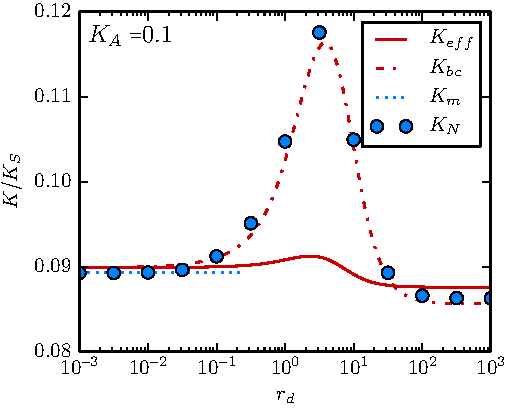
\includegraphics[width = 1 \textwidth]{plots/rep_rate_comparison0.pdf} \\
        \hspace{-1cm } 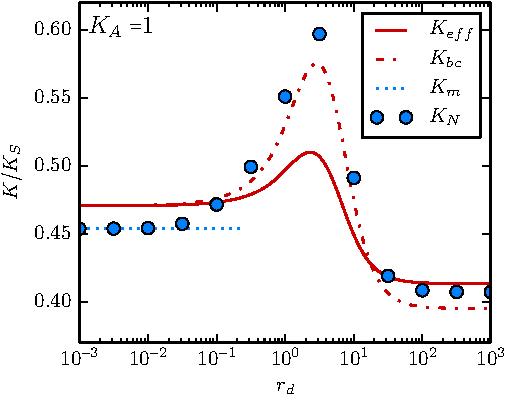
\includegraphics[width = 1 \textwidth]{plots/rep_rate_comparison1.pdf} \\
        \hspace{-1cm } 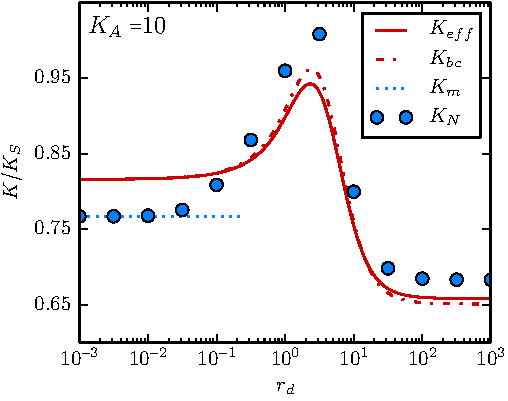
\includegraphics[width = 1 \textwidth]{plots/rep_rate_comparison2.pdf}
    \end{figure}
\end{minipage}
\begin{minipage}[t]{.37 \textwidth}
    \begin{figure}[H]
        \caption{Reaction rates for a nonideal sink with surface reaction rate $K_A$. Comparison of different analytic aproaches to numeric results obtained by the Method of lines \ref{method_of_lines}. The exact procedures are described in section \ref{Assumption2}. The potential is of the form given by equation \eqref{generalized_gaussian} with $n = 32$. Other parameters are given in table \ref{Parameters} and the surface reaction rate of the sink as defined by equation \eqref{Nonideal_sink_BC} is stated for each plot explicitly.\label{Rho_numeric}} 
    \end{figure}
    In this case also the assumption of independence of the diffusion controlled rate over the fluctuating barrier and the surface reaction rate breaks down as can be seen from the mismatch of $K_{eff}$ and $K_{bc}$. What is curious is that for decreasing surface reaction rate $K_A$ the solution for the ideal step shaped barrier does produce very good results in terms of reaction rates even in the fast switching limit to the effect that they are in god agreement with the numeric result for smooth barriers. Bearing in mind the discussion about the fast switching limit in section \ref{Numeric_Study} it is not clear whether this is only a coincidence or not. To make this clear it would be necessary to examine the \end{minipage}



\section{Fundamentals and Methods}
\label{Short_Introduction_to_Stochastic_Processes}
This section will introduce some basic concepts and fundamentals of stochastic processes and reaction rate theory as they concern the problem under study. For a broader context please refer to standard textbooks \cite{VanKampen1992} or review papers on the topic \cite{Calef1983a, Bressloff2013}. The goal here is to give a framework for the treatment of multivariate Markov processes in discrete and continuous space and to present the reference case for diffusion controlled reactions rates in the Debye-Smoluchowski interpretation \cite{Smoluchowski1917a, Debye1942}. \\
Therefore we take the well-trodden trail from the Chapman Kolmogorow equation via the Kramers Moyal expansion to the Kolmogorow forward or Fokker-Planck equation. Here we take a step to the side to calculate the drift and diffusion coefficients from the Langevin equation in the 'overdamped' case of a Brownian particle before we show the derivation of the Master equation again from the Chapman-Kolmogorow equation.\\
Thereafter we use the methods introduced before to illustrate the treatment of multivariate Markov processes in discrete and continuous space. \\
Finally we show a rigorous derivation of the diffusion controlled reaction rate from the Fokker-Planck description of a spherical sink embedded in a bath of Brownian particles.
\subsection{The Fokker Planck Equation}
\label{The_Fokker_Planck_Equation}
Brownian motion is a Markovian process, i.e. each time step in the random motion of particles does only depend on their preceding position. This implies, that the conditional probability density function (PDF) of their coordinates obeys the following relation:
\begin{equation}
    p(x_{3},t_{3}|x_{2},t_{2};x_{1},t_{1}) = p(x_{3},t_{3}|x_{2},t_{2}), \quad t_{3}>t_{2}>t_{1}
    \label{}
\end{equation}
This relation implies, that for a Markov process every multi step probability distribution can be expressed as a hierarchy of a initial distribution and the two step transition probabilities. For $ t_1 < t_2 < \cdots < t_n$:
\begin{align}
    p(x_1,t_1;x_2,t_2;\cdots;x_n,t_n) &= p(x_n,t_n|x_{n-1},t_{n-1})P(x_{n-1},t_{n-1}|x_{n-2},t_{n-2}) \cdots \nonumber \\
                                      & \cdots p(x_2,t_2|x_1,t_1)p(x_1,t_1)
    \label{hierarchy}
\end{align}
So the entire realization of the process is determined by the initial distribution and the two step transition probability. \\
Integrating the three step joint probability distribution over the intermediate step leads to the Chapman Kolmogorow equation
\begin{equation}
    p(x_3,t_3|x_1,t_1) = \int p(x_3,t_3|x_2,t_2) p(x_2,t_2|x_1,t_1) {\rm d} x_2.
    \label{Chapman Kolmogorov equation}
\end{equation}
From the Chapman Kolmogorow equation we will derive the Kramers Moyal expansion. Therefore we multiply  with $p(x_1,t_1)$ and integrating over $x_1$ which leads to
\begin{equation}
    p(x_3,t_3) = \int p(x_3,t_3|x_2,t_2)p(x_2,t_2) {\rm d} x_2.
    \label{ck3}
\end{equation}
The integrand may be written in terms of $\Delta x = x_3 - x_2$ and then be expanded for $\Delta x << 1$
\begin{align}
    p(x_3,t_3|x_2,t_2)p(x_2,t_2) &= p( (x_3 - \Delta x) + \Delta x, t_3|x_3 - \Delta x, t_2)p( (x_3 - \Delta x), t_2) \nonumber \\
    &= \sum_{n=0}^{\infty} \frac{(-1)_{n}}{n!}\frac{\partial^{n}}{\partial x_3^{n}}\left\{p(x_3 + \Delta x, t_3|x_3,t_2) p(x_3,t_2)\right\}
\end{align}
Inserting again in \eqref{ck3} integrating over $\Delta x$ and substituting $\Delta t = t_3 - t_2$ yields
\begin{equation}
    p(x_3,t_2 + \Delta t) = \sum_{n=0}^{\infty} \frac{(-1)_{n}}{n!}\frac{\partial^{n}}{\partial x_3^{n}}\left\{ M_{n}(x_3,t,\Delta t) p(x_3,t_2) \right\}
    \label{KM1}
\end{equation}
where $M_n$ are the so called \textit{jump moments} defined by
\begin{equation}
    M_n(x,t,\Delta t) = \int (\Delta x)^{n} p(x + \Delta x, t + \Delta t | x, t) {\rm d} (\Delta x).
    \label{Jump_moments}
\end{equation}
Since $p(x+\Delta x, t|x,t) = \delta (\Delta x)$ it follows from the definition of the jump moments, that $\lim_{\Delta t \rightarrow 0} M_{n}(x,t,\Delta t) = 0$ for $n > 1$. Also $M_{0}(x,t,\Delta t) = 1$. Bearing this in mind, we now assume, that the jump moments can be expanded for $n > 1$ and small $\Delta t$
\begin{equation}
    M_{n}(x,t,\Delta t) = K^{(n)}(x,t)\Delta t + O(\Delta t^{2}).
\end{equation}
Substituting this into equation \eqref{KM1}, dividing by $\Delta t$ and taking the limit $\Delta t \rightarrow 0$ results in 
\begin{equation}
    \frac{\partial p(x,t)}{\partial t} = \sum_{n = 1}^{\infty}\frac{(-1)^{n}}{n!}\frac{\partial^n}{\partial x^n} \left\{ K^{(m)}(x,t) p(x,t) \right\}.
    \label{Kramers Moyal expansion}
\end{equation}
The so called Kramers-Moyal coefficients $K_{n}(x,t)$ can be calculated from the transition probability $T_{\Delta t}(x,\Delta x,t) = p(x+\Delta x,t+\Delta t | x, t)$:
\begin{equation}
    K^{(n)}(x,t) = \lim_{\Delta t \rightarrow 0} \frac{1}{\Delta t} \int {\rm d}(\Delta x) T_{\Delta t}(x,\Delta x,t) (\Delta x)^m .
    \label{jump moments}
\end{equation}
So far nothing has be assumed, other than the Markov property and the existence of the Taylor series. However in many application the examination of the jump moments reveals, that it is a suitable approximation to truncate the expansion for $n>2$. In this case, one obtains the following form, known as the \textit{Fokker Planck equation}   
If the expansion is truncated after the second term, the result gives the well known Fokker Planck Equation:
\begin{equation}
    \frac{\partial p(x,t)}{\partial t} = - \frac{\partial}{\partial x} \left[A(x,t)p(x,t) \right] + \frac{1}{2}\frac{\partial^2}{\partial x^2}\left[ B(x,t)p(x,t) \right] 
    \label{FPE}
\end{equation}
where $A$ and $B$ are independent of $t$ if the process is stationary. \\
\subsection{Brownian Motion}
\label{Brownian_Motion}
Brownian motion is the oldest example of a Markov process that is known in physics. A heavy particle in a solution of lighter particles, which collide with it in a random fashion. Consequently, the velocity of the heavier particle undergoes a series of supposedly uncorrelated jumps. When the velocity $v$ has a certain direction, there will be on average more collisions from this side, than from the other. Therefore the probability of a change in velocity $\Delta v$ depends on its current value, but not on the velocity at earlier times. As a consequence, the velocity of the heavier particle can be considered to be a Markov process. When the whole system is in equilibrium the process is stationary and its autocorrelation time is the time in which an initial velocity is damped out. \\
Now in the \textit{overdamped limit} the correlation time of the velocity is much smaller then the time between two observations of the heavy particle. In that case the observation of the particle gives a series of positions $x(t_1), x(t_2) \cdots$. Each displacement $x(t_{i+1}) - x(t_{i})$ does not depend on the previous history of the process, i.e. it is independent of $x_{i=1}, x_{i-2}\cdots$. Hence not only the velocity, but also the position of the particle is a Markov process (at least on a coarse grained timescale). 
\par
In the following we will start with the Langewin equation for the velocity of a particle in a fluid and derive the corresponding Kramers Moyal coefficients to obtain a Fokker-Planck equation for the distribution of its position. 

\begin{equation}
    m \frac{{\rm d}^2 x}{{\rm d}t^2} = -\gamma \frac{ {\rm d}x}{{\rm d}t} + f(x) + \varepsilon(t)
    \label{Langewin equation}
\end{equation}
Here $\varepsilon(t)$ is a Gaussian distributed random process describing the collision interaction of the particle and the solute. $f(x)$ is a force resulting from an external potential and is taken to be independent of $t$. It can be shown, that the correlation time of this process is $\tau = \dfrac{m}{\gamma}$. In the so called overdamped limit $ \tau >> 1$ this equation results in
\begin{equation}
    \gamma \frac{ {\rm d}x}{{\rm d}t} = f(x) + \varepsilon(t)
    \label{BD1}
\end{equation}
As described in the introductory part the process must be observed on a coarse grained timescale to be considered Markovian. Therefore the expression can be discretized in time and transforms to:
\begin{equation}
        x(t + \Delta t) = x(t) + \frac{1}{\gamma}f(x,t) \Delta t + \frac{1}{\gamma} \varepsilon'(t) \Delta t.
    \label{overdamped limit}
\end{equation}
with the distribution of the random force being
\begin{equation}
    P(\varepsilon ' ) = \sqrt{\frac{\Delta t}{4 \pi D \gamma^{2}}} \exp \left[ - \frac{\varepsilon ^{\prime 2} \Delta t}{4 D \gamma^{2}} \right].
    \label{eps dist}
\end{equation}
From this distribution one can compute the transitions probability for the Brownian particle as:
\begin{align}
    T_{\Delta t}(x,\Delta x,t)  &= \left< \delta \left(  \Delta x - (x(t-\Delta t) - x(t)) \right)\right> \nonumber\\
                        &= \int \rm{d}\varepsilon ' \delta \left(  \Delta x - (x(t-\Delta t) - x(t)) \right)  \sqrt{\frac{\Delta t}{4 \pi D \gamma^{2}}} \exp \left[ - \frac{\varepsilon  ^{\prime 2} \Delta t}{4 D \gamma^{2}} \right] \nonumber\\
                        &= \sqrt{\frac{1}{4 \pi D \Delta t}} \exp \left[ \frac{-\left(\Delta x - f(x) \frac{\Delta t}{\gamma} \right)^2}{4 D \Delta t} \right]
    \label{T}
\end{align}
For this Gaussian transition probability the coefficients of the Kramers Moyal Expansion vanish after the second term, such that the resulting Fokker Planck equation holds the full analytic solution for the time evolution of the distribution of particles.
\begin{equation}
    \frac{\partial p(x,t)}{\partial t} = - \frac{\partial}{\partial x} \left[f(x)p(x,t) \right] + D\frac{\partial^2}{\partial x^2}\left[p(x,t) \right] 
    \label{FPE2}
\end{equation}

\subsection{The Master-Equation}
\label{The_Master_Equation}
The master equation is an equivalent formulation of the Kramers Moyal expansion for a certain class of stochastic processes. Namely those, whose transition probability has the following behaviour in the limit of small time steps $\Delta t$:
\begin{equation}
    p(x_2,t+\Delta t|x_1,t) = W(x_2|x_1)\Delta t + \left[ 1 - \Delta t \int {\rm d} x W(x_2|x_1) \right] \delta(x_2-x_1) + O(\Delta t ^{2})
    \label{master assumption}
\end{equation}
This assumption has the following meaning: The system was in state $x_1$ at time $t$ and made a transition to state $x_2$ during the time $\Delta t$. Then the probability of the transition is expressed in terms of the (non negative) {\it transition rate} i.e. the transition probability per unit time $W(x_2|x_1)$. To maintain a readable form we introduce the notation $T_\tau (x_2|x_1) = p(x_2,t+\tau|x_1,t)$ and omit the absolute time dependence, since the process is assumed to be stationary. \\
Using the Chapman-Kolmogorov equation it follows that
\begin{equation}
    T_{\tau + \tau'}(x_3|x_2) = \int T_{\tau'}(x_3|x_2)T_{\tau}(x_2|x_1){\rm d} x_2,
    \label{K2}
\end{equation}
and thus:
\begin{equation*}
    T_{\tau+\tau'}(x_3|x_1) = \int \left\{ \left[1 - \tau' \int {\rm d} z W(z|x_3) \right] \delta(x_3 - x_2) + \tau' W(x_3|x_2) \right\} T_{\tau}(x_2|x_1){\rm d} x_2
\end{equation*}
Regrouping the terms and dividing by $\tau ' $ leads to:
\begin{align*}
    \frac{1}{\tau'} T_{\tau+\tau'}(x_3|x_1) &= \frac{1}{\tau'}  \int T_{\tau}(x_2|x_1) \delta(x_3 - x_2){\rm d} x_2\\
    &- \int \left\{ W(z|x_2)  T_{\tau}(x_2|x_1)\delta(x_3 - x_2) \right\}{\rm d} z {\rm d} x_2 \\
    &+ \int \left\{ W(x_3|x_2) T_{\tau}(x_2|x_1) \right\}{\rm d} x_2
\end{align*}
which in the limit of $\tau' \rightarrow 0$ leads to the desired master equation:
\begin{equation}
    \frac{\partial}{\partial \tau}T_{\tau}(x_3|x_1) = \int \left\{ W(x_3|x_2) T_{\tau}(x_2|x_1) - W(x_2|x_3) T_{\tau}(x_3|x_1) \right\}{\rm d} x_2
    \label{continuous_space_master_equation}
\end{equation}
where the $W(x_i|x_j)$ are properties of the specific process.
This equation describes the time development of the transition probabilities given an initial condition $(x_1,t_1)$. A more intuitive form follows from multiplying and integrating over a distribution of initial conditions $p(x_1,t_1)$ and its spatial coordinate $x_1$.
\begin{equation}
    \frac{\partial p(x,t)}{\partial t} = \int \left\{ W(x|x') p(x',t) - W(x'|x)p(x,t) \right\} {\rm } x'
\end{equation}
In this form the meaning becomes particularly clear. The master equation is a \textit{gain loss equaition} for the probabilities of each state $x$. The first term on the rhs. describes the gain of probability of state $x$ due to transitions from other states $x'$, whereas the second term on the lhs. describes the loss of probability of state $x$ due to transitions to other states.\\
For a discrete state space, the master equation has the form of a system of coupled ordinary differential equations:
\begin{equation}
    \frac{{\rm d} p_n(t)}{{\rm d} t} = \sum_{n'} W_{n n'}p_{n'}(t) - W_{n'n}p_{n}(t)
    \label{discrete_space_master_equation}
\end{equation}
$W$ is called a transition rate matrix and satisfies the following conditions:
\begin{align*}
    &0 \ge W_{n,n'} \quad \mbox{ for all } n \ne n' \\
    &0 \ge -W_{n,n} \ge \infty \\
    &\sum_{n'} W_{n,n'} = 0
    \label{Transitions_rate_matrix}
\end{align*}
In general it is not symmetric and can thus not be diagonalized. \\
From eq. \eqref{discrete_space_master_equation} one immediately sees, that for a steady state solution this implies, that the loss of probability from one state is compensated by the gain of probability by transitions from other states.\\
For stationary time reversible Markov processes this criterion can even be tightened to a property called \textit{detailed equilibrium}.
This property requires, that the total amount of probability going from two states in to each other must be equal i.e.
\begin{equation}
     W_{n n'}p_{n'} = W_{n'n}p_{n}
    \label{detailed_balance}
\end{equation}
This property implies a certain symmetry of the matrix and can be used to show, that for this class of transition rate matrices can be transformed to a symmetric state such that they can be diagonalized via a suitable orthogonal transformation.
\subsection{Multivariate Markov Processes}
\label{Multivariate_Markov_Processes}
It is straight forward to continue to Markov processes whose sample space is a direct product of continuous and discrete variables i.e. $\Omega = \mathbb{R}^{3} \times [1,\cdots, N]$. The Chapman Kolmogorov equation then becomes
\begin{equation}
    p(\vec{x}_3,n_3,t_3|\vec{x}_1,n_1,t_1) = \sum_{n_2} \int p(\vec{x}_3,n_3,t_1|\vec{x}_2,n_2,t_2)p(\vec{x}_2,n_2,t_2|\vec{x}_1,n_1,t_1) {\rm d} \vec{x}_2
    \label{MCK}
\end{equation}
In this case the variable $\vec{x}$ can be treated by the approach discussed in section \ref{The_Fokker_Planck_Equation} whereas the variable $n$ will be treated by the approach described in section \ref{The_Master_Equation}. This leads to a combined Master Fokker-Planck equation for the time evolution of the pdf
\begin{align}
    \frac{\partial}{\partial t } p(\vec{x},n,t) =   &- \vec{ \nabla } \left[\vec{A}(\vec{x},n,t)p(\vec{x},n,t) \right] + \frac{1}{2}\vec{\nabla}^{2}\left[ B(\vec{x},n,t)p(\vec{x},n,t) \right] \nonumber \\
                                                    &+ \sum_{n'} \left\{ W_{nn'}p(\vec{x},n',t) - W_{n'n}p(\vec{x},n,t)\right\}
    \label{fpmeq1}
\end{align}
It is convenient to write this equation in a vector notation for the variable $n$ indicating with $\vect{p}$ the vector $(p(0),p(1),\cdots,p(N))$ the vector on the $N$ dimensional space over the closed interval $[0,1]$ (the variables $\vect{x}$ and $t$ have been omitted). \\ 
Therefore we introduce a diagonal Fokker-Planck operator for the drift and diffusion terms
\begin{equation}
    \mathbb{F} = - \vec{ \nabla } \vec{A}(\vec{x},n,t) + \frac{1}{2}\vec{\nabla}^{2} B(\vec{x},n,t)
    \label{fpo}
\end{equation}
and write the transition rate matrix as $\mathbb{W}$ as
\begin{align*}
    &\mathbb{W}_{n,n'} = W_{nn'} \mbox{ for } n \ne n' \mbox{ as in eq. \eqref{discrete_space_master_equation}} \\
    &\mathbb{W}_{nn} = -\sum_{n \ne n'}W_{nn'}
\end{align*}
such that eq. \eqref{fpmeq1} has the following more compact form
\begin{equation}
    \frac{\partial}{\partial t} \vect{p}(\vec{x},t) = \left\{ \mathbb{F} + \mathbb{W} \right\} \vect{p}(\vec{x},t).
    \label{fpmeq2}
\end{equation}

\section{The Smoluchowski Reaction Rate}
For educational reasons and since we will refer to it later, we will at this point give the solution to the original Smoluchowski problem.
The problem involves a perfect spherical sink of radius $R_s$ embedded in an initially homogeneous distribution of Brownian particles. The aim is to calculate the time dependent and stationary absorption rate of particles into the sink.
The boundary and initial conditions are therefore
\begin{align}
    \rho(r > R_s, t = 0) &= \rho_o, \\
    \rho(r=R_s,t) &= 0, \\
    \lim_{r \rightarrow \infty} \rho(r, t) &= \rho_o.
    \label{BC}
\end{align}
In the following, the corresponding Fokker Planck Equation in terms of particle densities
\begin{equation}
        \frac{\partial \rho(\vec{r},t)}{\partial t} = - \vec \nabla \left[ \vec f(\vec{r})\rho(\vec{r},t) \right] + D\vec \nabla ^2 \left[\rho(\vec{r},t) \right] 
    \label{FPE3}
\end{equation}
will be solved without external force, i.e. $\vec f(r) = 0$ and subject to the given boundary and initial conditions.
With the substitution $r \cdot \rho(r,t) = u(r,t)$ and the assumption, that the problem is spherically symmetric the derivatives in the Fokker Planck equation simplify to
\begin{equation}
    \frac{\partial u(r,t)}{\partial t} = D \frac{\partial ^2 u(r,t)}{\partial r^2}
    \label{Simplified FPE}
\end{equation}
Laplace transform of the equation yields:
\begin{align}
    \int_0^\infty e^{-st}\frac{\partial u(r,t)}{\partial t} \rm{d} t &= D \frac{\partial ^2 }{\partial r^2} \int_0^\infty e^{-st} u(r,t) \rm{d} t \\
    \left[e^{-st} u(r,t) \right]_0^\infty + s \int_0^\infty e^{-st} u(r,t) \rm{d} t &= D \frac{\partial^2}{\partial r^2} \tilde{u}(r,s)\\
    u(r,0) + s \tilde{u}(r,s) &= D \frac{\rm{d}^2}{\rm{d} r^2} \tilde{u}(r,s).
\end{align}
This is an ordinary 2nd degree inhomogeneous differential equation with constant coefficients.
For the standard ansatz $\tilde{u}(r,s) = \exp(\lambda(s) r)$ for the homogeneous solution we get the following characteristic polynomial:
\begin{equation}
    \lambda(s) ^2 - \frac{s}{D} = 0
    \label{characteristic_polynomial}
\end{equation}
resulting in the following homogeneous solution:
\begin{equation}
    \tilde{u}_h(r,s) = C_1 e^{ - \sqrt{\frac{s}{D}} \cdot r } + C_2 e^{ \sqrt{\frac{s}{D}} \cdot r }
    \label{u_h}
\end{equation}
We find the inhomogeneous solution using a polynomial ansatz of the form $\tilde{u}_i = C_3 r + C_4$ leading to the following relation:
\begin{align}
    s(C_3 r + C_4)  &= -u(r,0)\\
                    &= - r \rho_o \\
    \Rightarrow C_3 &= \frac{r}{s}\rho_o \\
                C_4 &= 0
\end{align}
Now the entire solution has to be fitted to the boundary conditions as in (\ref{BC}). The solution in Laplace space then reads:
\begin{equation}
\tilde{u}(r,s) = \rho_o \left( \frac{r}{s} + \frac{R_s}{s} e^{ \sqrt{\frac{s}{D}}(R_s - r) } \right) 
\end{equation}
The inverse Laplace transform
\begin{align}
    u(r,t)  &= \frac{1}{2 \pi i} \int\limits_{\gamma - i \infty}^{\gamma + i \infty}  e^{st} \tilde{u}(r,s){\rm d}t \\
    &= \frac{\rho_o}{ 2 \pi i} \left\{  \int\limits_{\gamma - i \infty}^{\gamma + i \infty} \frac{r}{s}  {\rm d}t +  \int\limits_{\gamma - i \infty}^{\gamma + i \infty}\frac{R_s}{s} e^{ \sqrt{\frac{s}{D}}(R_s - r) }  {\rm d}t \right\}
    \label{inverse laplace}
\end{align}
is done using the residue theorem for the first integral:
\begin{align}
    \oint_{ \gamma } {\rm d}z f(z) &= 2 \pi i \sum_{k = 1}^{n}I(\gamma, a_k) {\rm Res}(f,a_k) \\
    { \rm Res}(f,y_o) &= \frac{1}{(m-1)!} \lim_{z\rightarrow z_o} \frac{{ \rm d} ^{m-1}}{{\rm d} z^{m-1}} \left[ (z - z_o)^{m}f(z) \right]
    \label{residue theorem}
\end{align}
and the following identity for the second:
\begin{equation}
    \mathcal{L}\left[ {\rm erfc\left( \frac{a}{2\sqrt{t}} \right)} \right] = \frac{1}{s}e^{a\sqrt{s}}
    \label{L(erfc)}
\end{equation}
resulting in the following time dependent solution for $u(r,t)$ resp. the particle density $\rho(r,t)$:
\begin{align}
    u(r,t) &= \rho_o \left\{ r - R_s {\rm erfc} \left( \frac{r - R_s}{\sqrt{4 D t}} \right) \right\} \\
    \rho(r,t) &= \rho_o \left\{ 1 - \frac{R_s}{r} + {\rm erf} \left( \frac{r - R_s}{\sqrt{4Dt}} \right) \right\}.
    \label{u(r,t)}
\end{align}
In the limit $t \rightarrow \infty$ this results in the steady state density profile:
\begin{equation}
    \rho(r) =  \rho_o \left( 1 - \frac{R_s}{r} \right)
    \label{steady_state_density}
\end{equation}
The reaction rate can be defined as the total flux of particles through the boundary $\Omega$ of the sink:
\begin{equation}
    K = \int_\Omega \vec{J} {\rm d}\vec{A} 
    \label{reaction rate}
\end{equation}
Using the differential continuity equation:
\begin{align}
    \frac{\partial \rho(\vec{r},t)}{\partial t}&= \vec{\nabla} \vec{J}(\vec{r},t) \\
    &= \vec{\nabla} \left\{ \rho(\vec{r},t) \nabla \vec{U}(\vec{r}) + D \vec{\nabla} \rho(\vec{r},t) \right\}
    \label{contiuity equation}
\end{align}
and the spherical symmetry of the solution one can derive the time dependent reaction rate of the Brownian particles with the spherical sink of radius $R_s$ as follows:
\begin{align}
    K(t) &= \int_\Omega D  \vec{\nabla} \rho(\vec{r},t) \\
    &= 4 \pi D R_s^2 \left. \vec{\nabla} \rho(\vec{r},t) \right|_{r = R_s}\\
    &= 4 \pi D R_s \rho_o \left( 1 + \frac{R_s}{\sqrt{4Dt}} \right)
    \label{ideal reaction rate}
\end{align}
Again in the limit of $t \rightarrow \infty$ this results in the steady state absorption rate:
\begin{equation}
    K = 4 \pi D R_s \rho_o
    \label{steady state ideal rate}
\end{equation}

\section{The Debye Reaction Rate}
\label{The_Debye_Reaction_Rate}
The problem of diffusion controlled reaction rates as outlined in the previous chapter was extended to interaction between the substrate and the absorbing particles. For the resulting Fokker-Plack Equation of the substrate particles
\begin{equation}
    \frac{\partial \rho(r,t)}{\partial t} = \vec \nabla \left[ \frac{\rho(r,t)\vec \nabla U(r)}{\gamma} + D \nabla \rho(r,t) \right]
    \label{fpe_debye}
\end{equation}
it is possible to obtain a steady state solution for the particle flux through the surface of the sink of radius $R_s$. Therefore one omits the lhs. and integrates the rhs. from $R_s$ to an arbitrary $r$. With $J$ being the particle flux
\begin{equation}
    \vec J(r,t) =  \frac{\rho(r,t)\vec \nabla U(r)}{\gamma} + D \nabla \rho(r,t)
    \label{flux}
\end{equation}
This results in
\begin{align}
    0 &= \int_{R_s}^{r} \vec \nabla \vec J(r) \nonumber \\
    \vec J(R_s) &=  \rho(r)\frac{\vec \nabla U(r)}{\gamma} + D \vec \nabla \rho(r).
\end{align}
Now since the absorption rate is given by the flux through the sink surface i.e. the flux $\vec J (R_s)$ integrated over the surface of the sink the rate $K$ is determined by the following equation:
\begin{equation}
    \frac{K}{4\pi D r^{2}} = \rho(r)\frac{\rm d}{\rm d r} \frac{U(r)}{K_B T} + \frac{\rm d}{\rm d r} \rho(r).
    \label{K}
\end{equation}
Equation \eqref{K} can be solved in terms of a general solution of the homogeneous differential equation
\begin{equation}
    \frac{\rm d}{\rm d r} \rho(r) = -\rho(r) \frac{\rm d}{\rm d r} \frac{U(r)}{K_B T}
    \label{homogeneous_equation}
\end{equation}
that has the form
\begin{equation}
    \rho(r) = C \exp \left[ - \frac{U(r)}{K_B T} \right].
    \label{homogeneous_solution}
\end{equation}
Using this the solution the inhomogeneous equation can be obtained by the method of variation of the constant. Therefore we take the constant $C$ in \eqref{homogeneous_solution} to be $r$ dependant and substitute $\rho(r)$ in eq. \eqref{K}:
\begin{align}
    \frac{K}{4 \pi D r^2} &= C(r) \exp \left[ - \frac{U(r)}{K_B T} \right] \frac{\rm d}{\rm d r} \frac{U(r)}{K_B T} + \frac{\rm d}{\rm d r} C(r) \exp \left[ - \frac{U(r)}{K_B T} \right] \nonumber\\
    \frac{K}{ 4 \pi D r^2} &= \exp \left[ -\frac{U(r)}{K_B T} \right] \frac{\rm d }{\rm d r} C(r)
    \label{equation_C(r)}
\end{align}
Now integrating this equation from $R_s$ to an arbitrary $r>R_s$ yields:
\begin{equation}
    C(r) = C(R_s) + \frac{K}{4 \pi D}\int_{R_s}^{r} \frac{\exp \left[ \frac{U(r')}{K_B T}\right]}{r'^2} \rm d r'
    \label{solution_C(r)}
\end{equation}
Using the boundary condition that $\rho(R_s)=0$  we can set the integration constant $C(R_s) = 0$ to obtain the result for the density profile of the substrate particles in the potential of the absorbing particle:
\begin{equation}
    \rho(r) = \frac{K}{4 \pi D}\exp \left[ -\frac{U(r)}{K_B T} \right] \int_{R_s}^{r} \frac{\exp \left[ \frac{U(r')}{K_B T}\right]}{r'^2} \rm d r'.
    \label{rho_debye}
\end{equation}
The rate $K$ can then be calculated by the use of the boundary condition that for $r \rightarrow \infty$ $\rho(r) \rightarrow \rho_o$ together with the assumption, that the interaction $U(r)$ only has a finite range, i.e. that it vanishes for $r \rightarrow \infty$:
\begin{equation}
    \rho_o = \lim_{r\rightarrow \infty} \rho(r) = \frac{K}{4 \pi D}\int_{R_s}^{\infty} \frac{\exp \left[ \frac{U(r')}{K_B T}\right]}{r'^2} \rm d r'
    \label{lim_rho_debye_infty}
\end{equation}
which is equivalent to 
\begin{equation}
    K = 4 \pi D \rho_o \left\{\int_{R_s}^{\infty} \frac{\exp \left[ \frac{U(r')}{K_B T}\right]}{r'^2} \rm d r' \right\}^{-1}
    \label{K_Debye}
\end{equation}
In the case of $U(r) \equiv 0$ this simplifies to the result obtained by Smoluchowski (comp. eq. \eqref{steady state ideal rate}.

\newpage
\section{Reaction Rates over Fluctuating Barriers}
\label{Reaction_Rates_over_Fluctuating_Barriers}
\subsection{Model Description}
\label{Model_Description}
The system under consideration consists of a spherical sink of radius $R_s$ that is surrounded by a potential barrier. The barrier is assumed to be of boxcar shape with limiting radius $a,b>R_s$. It fluctuates between states $n$ with different hight $U_n \in [U_0, \cdots U_N]$ subject to a transition rate matrix $\mathbb{W}$. The system is embedded in a reservoir of Brownian particles. It is desired to find the rate at which the particles are absorbed by the sink, given that the transition rate matrix of the potential fluctuations satisfies the detailed balance property.\\
The appropriate boundary conditions are, that the probability density function of the Brownian particles is zero at $R_s$ and takes a constant finite value for $|\vec{r}| \rightarrow \infty$. Due to the fact that the system is not spatially bounded it is not possible to normalize the joint pdf $\vect{p}(\vec{r},n,t)$ of the position of the Brownian particles and the state of the potential barrier in the sense that 
\begin{equation}
    \sum_n \int_{\mathbb{R}^{3}} p_n(\vec{r},t) {\rm d}V = 1.
    \label{pdfNormalization}
\end{equation}
Instead it is appropriate to normalize the distribution to the particle density $\vect{\rho}(\vec{r},t)$ as commonly done in statistical physics
\begin{equation}
    \sum_n \int_V \rho_n(\vec{r},t) {\rm d}V = N
    \label{densNormalisation}
\end{equation}
where $N$ is the total number of particles enclosed in the volume $V$. The time evolution of the joint pdf can be described by eq. \eqref{fpmeq2} derived in the previous section
\begin{equation}
    \frac{\partial}{\partial t}\vect{\rho}(\vec{r},n,t) = \left\{ \mathbb{F} + \mathbb{W} \right\} \vect{\rho}(\vec{r},n,t).
    \label{fpmeq3}
\end{equation}
Using the spherical symmetry of the system, the Fokker-Planck operator can be written as
\begin{equation}
    \mathbb{F} = {\rm diag}\left[ \vec{\nabla}\frac{1}{\gamma}\left( \vec{\nabla} U_n(r) \right)+ D \vec{\nabla}^{2} \right].
    \label{fpo2}
\end{equation}
It becomes obvious from this equation, that the state of the potential might as well be seen as a property of the Brownian particles. One could for instance imagine the barrier as a constant electric potential. Then the particles are fluctuating between differently charged states. For the assumption of noninteracting particles to be still valid, the solution has to be dilute and the Debye screening length has to be small. \\
\subsection{Fit Conditions}
\label{Fit_Conditions}
For the boundary at $|\vec{r}| \rightarrow \infty$ far away from the influence of the potential and the sink it is reasonable to assume that the particle density distribution is a stationary solution $\vect{\rho}^{(eq)}$ the sole Master equation. From the assumption of detailed balance it follows that it has to satisfy
\begin{align}
    &\mathbb{W} \vect{\rho}^{(eq)} = 0 \nonumber \\
    &\mathbb{W}_{n'n} \rho_n^{(eq)} = \mathbb{W}_{nn'}\rho_{n'}^{(eq)}.
    \label{detailed_balance2}
\end{align}
It can be shown that this $\vect{\rho}^{(eq)}$ is not degenerate and that all its entries are positive. \\
The next issue to investigate is the behaviour of the steady state solution for the particle density distribution at the jump discontinuities of the potential 
\begin{equation}
  U_n(r) = \left\{ \begin{array}{l l} 
        0 &: R_s < r \le a \\
        U_n &: a<r \le b \\
        0 &: b < r \le R_d
    \end{array} \right.
    \label{step_potential}
\end{equation}
Therefore we first integrate from the boundary of the sink to some arbitrary $r > R_s$
\begin{equation*}
    \int_{R_s}^{r}\mathbb{F}\vect{\rho}(r'){\rm d} r' = - \mathbb{W} \int_{R_s}^{r} \vect{\rho}(r') {\rm d} r' .
\end{equation*}
Note that the lower boundary of the Integral on the lhs is proportional to the particle flux through the sink boundary whereas the upper bound is proportional to the particle flux through the surface of a sphere with radius $r$ at a certain state of the potential. The Integral on the rhs is proportional to the particle flux from and to the this state of the potential in the observed volume due to transitions from and to other states of the potential.\\
    \begin{equation}
        \frac{1}{\gamma}\rho_n(r) \vec{\nabla} U_n(r) + D \vec{\nabla} \rho_n(r) = J_n(R_s) - \left\{ \mathbb{W} \int_{R_s}^{r} \vect{\rho}(r') {\rm d} r' \right\}_{n}
    \end{equation}
Now we integrate over a small vicinity of the jump discontinuity with width $\varepsilon$ and take the limit of $\varepsilon \rightarrow 0$
    \begin{equation}
        \int_{a-\varepsilon}^{a + \varepsilon} \frac{U_n}{\gamma D}\delta(a-r) + \int_{a-\varepsilon}^{a + \varepsilon} \frac{1}{\rho_n(r)}\nabla \rho_n(r) = \underbrace{\int_{a - \varepsilon}^{a + \varepsilon}\frac{J_n(r)}{\rho_n(r) D} - \int_{a - \varepsilon} ^{a+ \varepsilon} \left\{ \mathbb{W} \vect{\rho}(r)\right\}_{n}}_\text{$O(\varepsilon)$}
    \end{equation}
Since the terms on the rhs. of the equation scale only with $\varepsilon$ we end up with a result previously known for systems in thermal equilibrium:
\begin{equation}
    \vect{\rho}^{(I)}(a) = \underbrace{ {\rm diag}\left[\exp\left\{\frac{U_n}{K_B T} \right\}\right]}_\text{\large$\mathbb{U}$} \vect{\rho}^{(II)}(a)
    \label{dens_fit}
\end{equation}
Here $\vect{\rho}^{(I)}$ and $\vect{\rho}^{(II)}$ refers to the particle density at different side of the jump discontinuity.
Analogously we find relations for the derivatives of the particle density at the jump discontinuity:
\begin{equation}
    \vec{\nabla}\vect{\rho}^{(I)}(a) = \vec{\nabla}\vect{\rho}^{(II)}(a)
    \label{ddens_fit}
\end{equation}
\subsection{Expansion in Eigenfunctions of $\mathbb{W}$}
\label{Expansion_in_Eigenfunctions}
The assumption of the detailed balance property that implies the existence of an equilibrium distribution $\vect{\rho}^{(eq)}$ allows for the definition of an operator $\mathbb{T}$
\begin{equation}
    \mathbb{T} = \delta_{n,n'} [\rho_n^{(eq)}]^{\frac{1}{2}}.
    \label{symmetrisation_transform}
\end{equation}
This is a similarity transform that symmetrises $\mathbb{W}$
\begin{equation}
    \mathbb{T}^{-1}\mathbb{W}\mathbb{T} = \mathbb{S}.
    \label{symm_rate_matrix}
\end{equation}
Using property \eqref{detailed_balance2} it follows that
\begin{align}
    \mathbb{S}_{il} &= \mathbb{T}^{-1}_{ij} \mathbb{W}_{jk} \mathbb{T}_{kl} = \sum_j \delta_{ij} [\rho^{(eq)}_i]^{-\frac{1}{2}} \mathbb{W}_{jk} \mathbb{T}_{kl} \\ \nonumber
    &= [\rho^{(eq)}_{i}]^{\frac{1}{2}} \sum_{k} \mathbb{W}_{ik} \delta_{kl} [\rho^{(eq)}_l]^{-\frac{1}{2}} = \mathbb{W}_{il}^{\frac{1}{2}} \left( \mathbb{W}_{il} \frac{\rho^{(eq)}_i}{\rho^{(eq)}_l} \right)^{\frac{1}{2}} \\ \nonumber
    &= \left(\mathbb{W}_{il} \mathbb{W}_{li}\right)^{\frac{1}{2}} \\ \nonumber
    S_{ii} &= W_{ii}.
\end{align}
The resulting matrix can then be diagonalized by an orthogonal matrix $\mathbb{D}$
\begin{equation}
    \mathbb{D}^{\dagger} \mathbb{S} \mathbb{D} = -{\rm diag}\left[ \lambda_i \right].
    \label{orthogonal_transform}
\end{equation}
It can be shown that $\lambda_i > 0$ for $i>1$ and $\lambda_1 = 0$ with the corresponding eigenvector
\begin{equation}
    D_{i1} = \rho^{(eq)}(i)^{\frac{1}{2}}.
\end{equation}
We now write equation \eqref{fpmeq3} in terms of eigenfunctions of $\mathbb{W}$
\begin{equation}
    \tilde{\vect{\rho}}(\vec{r},t) = \mathbb{A}^{-1} \vect{\rho}(\vec{r},t)
    \label{eigenfunctions}
\end{equation}
where $\mathbb{A}$ denotes the transformation $\mathbb{T}\mathbb{D}$ and use the fact that the potential term vanishes everywhere but at the jump discontinuities. Therefore equation \eqref{fpmeq3} reads
\begin{equation}
    \frac{\partial }{\partial t} \tilde{\vect{\rho}}^{(j)}(\vec{r},t) = {\rm diag} \left[D \vec{\nabla}^{2} - \lambda_i  \right] \tilde{\vect{\rho}}^{(j)}(\vec{r},t)
    \label{fpmeq4}
\end{equation}
For the steady state case where the lhs. vanishes it it straight forward to write down the solution to this equation
\begin{align}
    \tilde{\rho}_{1}^{(j)}(r) &= c_{1,1}^{(j)} + c_{1,2}^{(j)} \frac{1}{r} \nonumber \\
    \tilde{\rho}_{i \ne 1}^{(j)}(r) &= c_{i,1}^{j}\frac{1}{r} \exp\left[-r\sqrt{\frac{\lambda_i}{D}}\right] + c_{i,2}^{j}\frac{1}{r} \exp\left[r\sqrt{\frac{\lambda_i}{D}}\right] 
    \label{fp_ind_sol}
\end{align}
Note that the solution corresponding to the first eigenvalue $\lambda_1 = 0$ equals the one derived in \eqref{steady_state_density} for the ungated problem. Together with the fitting conditions obtained in \eqref{dens_fit} they would result in the solution for a constant boxcar shaped potential barrier. \\
The other solutions corresponding to the nonzero eigenvalues of the transition rate matrix $\lambda_i<0$ describe deviations from this solution due to the metastability of the potential barrier. Note that they exponentially decay in space with a \textit{decay length}
\begin{equation}
    r_d^{(i)} = \sqrt{\frac{\lambda_i}{D}}
    \label{decay_length}
\end{equation}
that is unique for each state of the potential and which is closely related to its decay rate in time.
\subsection{Treatment of Boundary and Fit Conditions}
\label{Treatment_of_Boundary_and_Fit_Conditions}
Now we have to find an expression, that allows for the calculation of the coefficients $c_{i,k}^{(j)}$ from the transformed boundary and fit conditions
\begin{align}
    \mathbb{A}^{-1}\vect{\rho}^{(I)}(R_s) &= \vect{\tilde{\rho}}^{(I)}(R_s) = 0 \nonumber \\
    \vect{\tilde{\rho}}(r \rightarrow \infty) &= \mathbb{A}^{-1} \vect{\rho}^{(eq)} = (1,0,\cdots,0)^{T}
\end{align}
and
\begin{align}
    \vect{\tilde{\rho}}^{(I)}(a) &= \mathbb{A}^{-1}\mathbb{U}\mathbb{A} \vect{\tilde{\rho}}^{(II)}(a), \\ \nonumber
    \vect{\tilde{\rho} '}^{(I)}(a) &= \vect{\tilde{\rho} '}^{(II)}(a), \\ \nonumber
    \vect{\tilde{\rho}}^{(III)}(b) &= \mathbb{A}^{-1}\mathbb{U}\mathbb{A} \vect{\tilde{\rho}}^{(II)}(b), \\ \nonumber
    \vect{\tilde{\rho} '}^{(III)}(b) &= \vect{\tilde{\rho} '}^{(II)}(b).
\end{align}
Therefore it is useful to write the solution of eq. \eqref{fpmeq4} as
\begin{equation}
    \tilde{\vect{\rho}}^{(j)} = \underbrace{ \left( \begin{array}{cllllllll}
       1   & \frac{1}{r}   & 0                 & 0                 & 0              & 0             & 0 & \cdots &\\
       0   & 0             &\frac{1}{r} e^{-r \alpha_2}   &\frac{1}{r} e^{r \alpha_2 }   & 0              & 0             & 0 & \cdots &\\
       0   & 0             & 0                 & 0                 &\frac{1}{r} e^{-r\alpha_3} &\frac{1}{r} e^{r\alpha_3} & 0 & \cdots &\\
       \vdots  &&&&&&&\ddots &\\
       \vdots  &&&&&&&&\ddots
   \end{array} \right)}_\text{\large$\hat{\rho}(r)$}
   \underbrace{\left(\begin{array}{c}  
       c_{1,1}^{(j)} \\ 
       c_{1,2}^{(j)} \\ 
       c_{2,1}^{(j)} \\ 
       c_{2,2}^{(j)}  \\ 
       \vdots 
   \end{array} \right)}_\text{\large$\mathbb{C}$}.
\end{equation}
Here $\alpha_i = (\lambda_i / D)^{1/2}$. Using this notation, the boundary and fit conditions can be but in one $6 N$ dimensional system of linear equations
\begin{equation}
    \left( \begin{array}{lll}
        \hat{\rho}(R_s) & 0 & 0 \\
        \hat{\rho}(a)   & -\tilde{\mathbb{U}}\hat{\rho}(a) & 0 \\
        \hat{\rho}'(a) & -\hat{\rho}'(a) & 0 \\
        0 &  -\tilde{\mathbb{U}}\hat{\rho}(b) & \hat{\rho}(b) \\
        0 &  -\hat{\rho}'(a) & - \hat{\rho}'(a) \\
        0 & 0 & \hat{\rho}(r\rightarrow \infty)
    \end{array}\right) \left( \begin{array}{c} c_{1,1}^{1} \\ \vdots \\ \vdots \\ \vdots \\ c_{N,2}^{3} \end{array} \right) = 
    \left( \begin{array}{c} 0 \\ \vdots \\ 0 \\ 1 \\ 0 \\ \vdots \end{array} \right) \begin{array}{c} \vdots \\ \vdots \\ \vdots \\ i = 5N+1 \\ \vdots \\ \vdots \end{array}
    \label{lgs}
\end{equation}
where dashes denote derivatives with respect to $r$. Solving this system of linear equations yields the somehow lengthy expressions for the coefficients $c_{i,k}^{(j)}$. \\ We obtain the actual density profile by applying the transformation $\mathbb{A}$ to return to the actual particle densities for the different states of the potential barrier.
\subsection{Calculation of Rates}
\label{Calculation_of_Rates}
The rate of the particles absorbed by the sink is calculated by taking the surface integral over the flux through the surface of the sphere with radius $R_s$
\begin{align}
    K   &= \int_{\partial \Omega_{R_s}} \vec{J} {\rm d} \vec{A}\nonumber\\
    &= \int_{\partial \Omega_{R_s}} D \vec{\nabla} \sum_{n=1}^{N} \rho_n^{(1)}(r)\nonumber \\
    &= 4 \pi D R_s^{2} \sum_{n=1}^{N} \left\{ \mathbb{A} \left. \frac{\partial}{ \partial r}\right|_{R_s} \tilde{\vect{\rho}} \right\}_n
    \label{Rate}
\end{align}
        So in the previous section 
\begin{itemize}
    \item We found fitting conditions for steady state density profiles at jump discontinuities of potential barriers,
    \item we propose a treatment for the fluctuations of the potential barrier in terms of eigenfunctions of its transition rate matrix assuming it satisfies a detailed balance property,
    \item we introduced a persistence length of the influence of the potential fluctuations on the particle density profile,
    \item and we provide a scheme for the calculation of the integration constants of the particle density functions.
\end{itemize}
Now that we have found a general way do derive an analytic solution we will investigate a simple example to reveal the qualitative implications of the previous work. 
\newpage



\chapter{An Illustrative Example}
\label{results}
This section will give a simple example of the previously described system to illustrate the implications of the barrier fluctuations coupled to the diffusive transport of Brownian particles.\\
It will also give a close examination of certain limits e.g. of very fast and very slow barrier fluctuations and compare these to simulation results. In addition, it will be evaluated, if the solution for a step shaped barrier is a valid approximation for smooth potentials of similar shape depending on the timescale of the barrier fluctuations. \\
\section*{A Two State Barrier with Symmetric Switching Rates}
\addcontentsline{toc}{section}{\numberline{}A Two State Barrier with Symmetric Switching Rates}
The simplest possible example for the system under study is that of a two state barrier that switches between one \emph{on} ($U_1 = 0$) and one \emph{off} ($U_2 \ne 0$) state symmetrically, i.e. the \emph{on} $\rightarrow$ \emph{off} and \emph{off} $\rightarrow$ \emph{on} rates are equal: 
\begin{equation}
    W_{1 2}=W_{2 1}=W
    \label{symmetric_rates}
\end{equation}
such that the potential of mean force acting on the Brownian particles is independent of the switching rate.
This allows for the detailed study of effects solely coming from the coupling of timescales between barrier fluctuations and diffusive transport without any other influence.
\section{Particle Density}
The first step for the investigation of the example is the calculation of the analytic solution for the density profiles of the Brownian particles. Therefore one first writes down the corresponding Fokker-Planck equation \eqref{fpmeq1} in terms of particle densities as outlined in section  \ref{Model_Description}. In this case it reads:
\begin{align}
    \frac{\partial \rho_1(r,t)}{\partial t} &= \vec \nabla \left[ D \vec \nabla \rho_1(r,t) \right] - W_{21}\rho_1(r,t) + W_{12}\rho_2(r,t) \nonumber \\
    \frac{\partial \rho_2(r,t)}{\partial t} &= \vec \nabla \left[\rho_2(r,t) \vec \nabla \frac{U_2(r)}{\gamma} + D \vec \nabla \rho_2(r,t) \right] - W_{12}\rho_2(r,t) + W_{21}\rho_1(r,t)
    \label{two_state_fpe}
\end{align}
Note that the particles in state $m=1$ move freely and are not subject to any potential barrier. 
Since the transition rates are symmetric as assumed in the introduction of this section \eqref{symmetric_rates} the transition rate matrix \eqref{transition_rate_matrix} consequently also has a symmetric form:
\begin{equation}
    \mathbb{W} = \left( \begin{array}{rr}
    W & -W \\
    -W & W 
\end{array} \right),
    \label{two_state_transition_matrix}
\end{equation}
and needs not to be symmetrized to calculated its eigenvalues by a suitable orthogonal transformation.
The eigenvalues are $\lambda_1 = 0$ and $\lambda_2 = -2W$ and steady state solution to the transition matrix, i.e. the eigenvector to its zero eigenvalue is: 
\begin{equation}
    \vect{\rho}^{(eq)}=\left(\frac{1}{2}, \frac{1}{2}\right)^{T}
    \label{rhoeq}
\end{equation}
which obviously satisfies the detailed balance property \eqref{detailed_balance}. \\
The diagonal form of equation \eqref{two_state_fpe} is now 
\begin{equation}
    \frac{\partial}{\partial t} \tilde{\vect{\rho}} = \left( \begin{array}{ll}
        D\vec{\nabla}^{2} & 0 \\
        0 & D\vec{\nabla}^{2} - 2W
    \end{array} \right) \tilde{\vect{\rho}}
    \label{fpmeq5}
\end{equation}
and the steady state solution \eqref{fp_ind_sol} in terms of eigenfunctions of $\mathbb{W}$ reads
\begin{align}
    \tilde{\rho}_1^{(k)} &= c_{1,1}^{(k)} + \frac{c_{1,2}^{(k)}}{r} \\
    \tilde{\rho}_2^{(k)} &= \frac{c_{2,1}^{(k)}}{r}{\rm exp}\left[-\frac{r}{r_d}\right]+ \frac{c_{2,2}^{(k)}}{r}{\rm exp}\left[\frac{r}{r_d}\right]
    \label{ind_sol_U2}
\end{align}
with the decay length $r_d$ defined in equation \eqref{decay_length}:
\begin{equation}
    r_d = \sqrt{\frac{D}{2W}}.
    \label{rd_two_state}
\end{equation}
Once the coefficients $c^{(k)}_{i,j}$ are calculated from the boundary and fit conditions the density profiles and the resulting reaction rate can be calculated from equation \eqref{decomposition} and \eqref{Rate}.
The solution depends on several parameters, namely the radius of the sink $R_s$, the barrier spacing $a$ and $b$, the hight of the potential barrier in the \emph{on} state and the decay length $r_d$. The first parameter that is studied is the decay length $r_d$. The easiest way to get a first impression of its influence is to look at the density profiles. Therefore several examples for different parameter choices are given in figure \ref{rsd} and \ref{asd}.
If not stated differently, the other parameters are given by the values in the following table.
\begin{equation}
    \begin{array}{r|l}
        Parameter & Value \\ \hline
        R_s & 1 \\
        a   & 6 \\
        b   & 11 \\
        U_2/K_B T & \mp 3 \\
    \end{array} 
    \label{Parameters}
\end{equation}
 The choice of parameters is arbitrary now since the influence of each of them will be examined separately in later parts of this section.
For illustrative reasons the total particle density is normalized to $\rho_{tot}^{(eq)}=2$ for $r \rightarrow \infty$ and the particle densities in the different states are depicted together with the mean particle density. \\
Since the state of the barrier can also be treated as a property of the Brownian particles as discussed in section \ref{Model_Description} it is convenient do so for the following discussion. The particles that are influenced by the barrier will hence be called \emph{active} whereas the particles that are not will be called \emph{inactive}. \\ In the density plots in figure \ref{rsd} and \ref{asd} the density of active particles is depicted in \textcolor{blue}{blue} while the density of the inactive particles is depicted in \textcolor{red}{red}. \\
In part A) of figure \ref{rsd} and \ref{asd} $r_d$ is much larger as the overall spacing of the potential barrier. In this case the particles in different states are mostly independent from each other. \\
In part C) $r_d$ of figures \ref{rsd} and \ref{asd} is much smaller than the spacing of the barrier. In this case the particle densities are equal except for a small around the barrier borders that is approximately $r_d$ wide.\\ 
This case neatly illustrates the role of $r_d$ as the persistence length of the influence of the potential fluctuations. For distances far (this means considerably greater that $r_d$) from the jump discontinuities of the potential at  $r=a,b$ the thermal motion of the Brownian particles dampens the influence of the potential barrier and the densities of active and inactive particles converge to the same value again.\\
The interesting behavior emerges if the decay length is approximately of the same order as the barrier spacing as visible in part B) of figures \ref{rsd} and \ref{asd}. Then the densities of the different particles species are not independent of each other over the entire width of the system. This somehow has the effect that the average particle density at the inside of the barrier unexpectedly high. \\
This is curious and worth a closer look. Therefore, in the following section the underlying mechanism of particle transportation and its implications on the reaction rate will be thoroughly examined. \\ 
\newpage


\begin{minipage}[t]{0.5 \textwidth}
    \begin{figure}[H]
        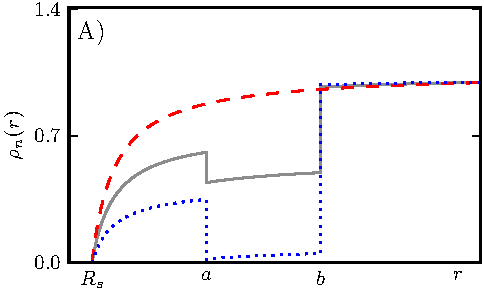
\includegraphics[width = 1 \textwidth]{plots/d1.pdf}
    \end{figure}
\end{minipage}
\begin{minipage}[t]{0.5 \textwidth}
    \begin{figure}[H]
        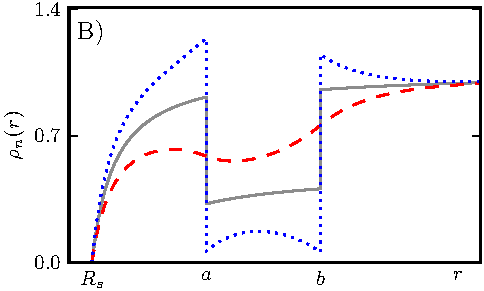
\includegraphics[width = 1 \textwidth]{plots/d2.pdf}
    \end{figure}
\end{minipage}
\begin{minipage}[t]{0.5 \textwidth}
    \begin{figure}[H]
        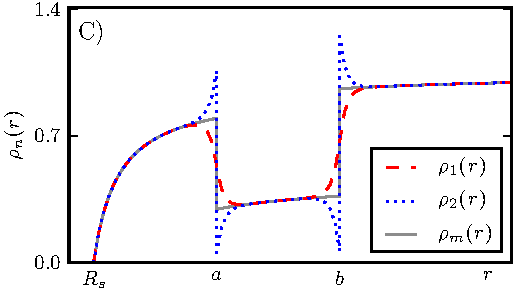
\includegraphics[width = 1 \textwidth]{plots/d3.pdf}
    \end{figure}
\end{minipage}\hspace{0.07\textwidth}\begin{minipage}[t]{0.43 \textwidth}
    \begin{figure}[H]
        \caption{Density profiles for repulsive fluctuating barrier. The densities of particles in state $m=1$ and state $m=2$ are depicted in dashed red, and dotted blue respectively. The decay length is given by A): $r_d = 250$, \newline B): $r_d=2.5$ and C): $r_d=0.25$. \label{rsd}}
    \end{figure}
\end{minipage}


\begin{minipage}[t]{0.5 \textwidth}
    \begin{figure}[H]
        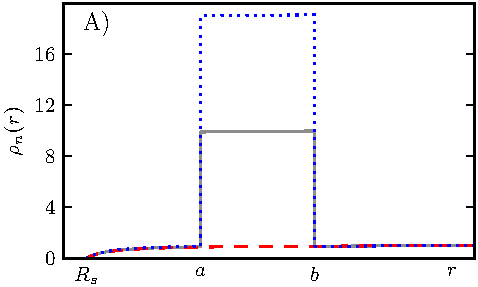
\includegraphics[width = 1 \textwidth]{plots/d4.pdf}
    \end{figure}
\end{minipage}
\begin{minipage}[t]{0.5 \textwidth}
    \begin{figure}[H]
        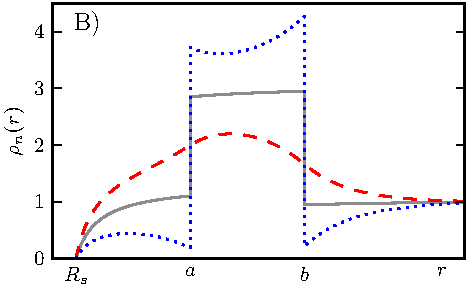
\includegraphics[width = 1 \textwidth]{plots/d5.pdf}
    \end{figure}
\end{minipage}
\begin{minipage}[t]{0.5 \textwidth}
    \begin{figure}[H]
        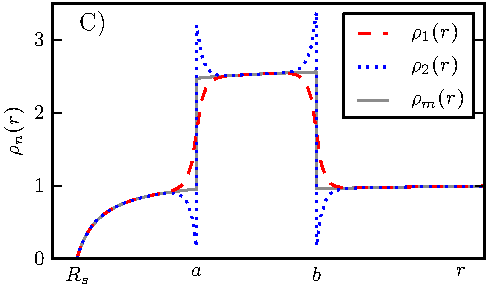
\includegraphics[width = 1 \textwidth]{plots/d6.pdf}
    \end{figure}
\end{minipage}\hspace{0.07\textwidth}\begin{minipage}[t]{0.43 \textwidth}
    \begin{figure}[H]
        \caption{Density profiles for attractive fluctuating barrier. The densities of particles in state $m=1$ and state $m=2$ are depicted in dashed red, and dotted blue respectively. The decay length is again given by A): $r_d = 250$, B): $r_d=2.5$ and C): $r_d=0.25$ \label{asd}}
    \end{figure}
\end{minipage} 
\newpage
\section{Flow Analysis}
\label{flow_analysis}
Density profiles only give information about where particles are. However, it is of interest how they got there and where they are going next. This is also necessary for the explanation of the behavior observed in part B) of figures \ref{rsd} and \ref{asd} in the previous section.
To investigate particle movement it is reasonable to use spatial and reactive fluxes for a further study of the system.
To do so the radial coordinate of the system is divided into different areas as depicted in figure \ref{fig:flowchart_scetch}.
\begin{figure}[H]
    \centering
    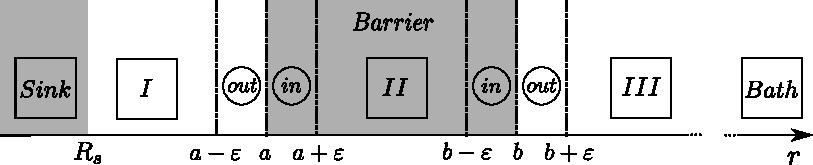
\includegraphics[width = .9 \textwidth]{plots/drawing.pdf}
    \caption{Sketch of the spatial discretization for the flow analysis of the system: The Sink and the Barrier are marked in gray. The circles represent narrow volumes of width $\varepsilon$ right at the barrier borders. $\varepsilon$ is set to be one tenth of the barrier width. The squares represent the remaining volumes between barrier and sink ($I$), between the barrier boundaries ($II$) and outside the sink ($III)$ . Each volume has the shape of a spherical shell (except the sink which is a sphere). Active and inactive particles are investigated separately in each of these volumes}
    \label{fig:flowchart_scetch}
\end{figure}
For each of these areas one examines the spatial fluxes from and to neighboring areas and the reactive fluxes from one particle state to the other. \\
For this purpose it is convenient to use the integral form of the continuity equation derived in \eqref{ce0}. To employ it in the actual problem one takes the density profiles to be constant in time such that its left hand side vanishes. Then the terms on the right hand side are calculated separately. The spatial fluxes at the volume boundaries:
\begin{equation}
    J_m^{(S)}(r_i) = \int_{r_i} \vec{j}_m(r) {\rm d} \vec{A}
    \label{spatial_flux}
\end{equation}
and the reactive fluxes from one particle species to the other:
\begin{equation}
    J_{mm'}^{(R)}(r_i,r_j) =\int_{r_i}^{r_j} \left\{ \mathbb{W}_{m'm}\rho_m - \mathbb{W}_{mm'} \rho_{m'} \right\} {\rm d} r
    \label{reaction_flux}
\end{equation}
where $r_i$ and $r_j$ are the radii $R_s$, $a-\varepsilon$, $a$ etc. of the spatial discretization given in figure \ref{fig:flowchart_scetch}.
These fluxes are then represented as arrows between the icons representing the corresponding areas as illustrated in figure \ref{fig:flowchart_scetch}. Active and inactive particles are depicted separately where the icons representing active particles are blue and the icons representing inactive particles are red. \\ \textbf{Interpreting the following flow diagrams it is important to note, that the flows depicted by the arrows are normalized to the largest value for each example. Therefore the arrows only represent \emph{relative importance of fluxes} and have no meaning for their absolute values!}
. \\ \vspace{-1.3 cm}

\begin{minipage}[t]{.372 \textwidth}
    \vspace{0.5 cm}
    \begin{figure}[H]
        \caption{Flow diagram for repulsive barrier: This plot shows spatial and reactive particle flows between different particle species (active particles are represented in blue, inactive particles are represented in red) and different spatial regions (see figure \ref{fig:flowchart_scetch} for reference) for the examples given in figure \ref{rsd}. The difference between the different plots is again the decay length which is equal to \newline A): $r_d=250$, B): $r_d=2.5$ and \newline C): $r_d = 0.25$.
    \label{fig:flow_repulsive}}
    \end{figure}
\end{minipage}\hspace{0.02 \textwidth}\begin{minipage}[t]{.608 \textwidth}
    \begin{figure}[H]
        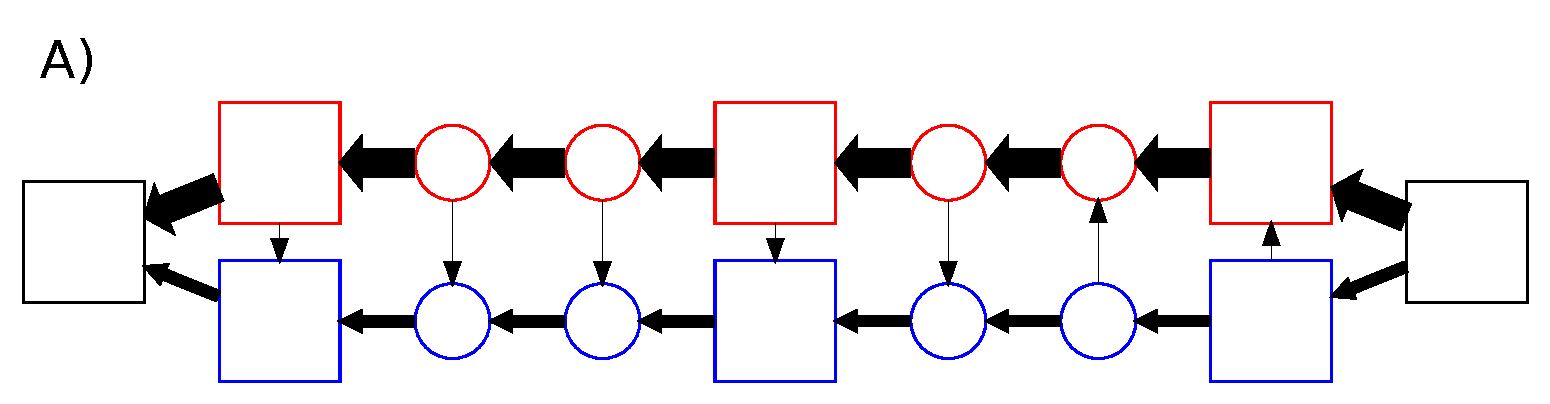
\includegraphics[width = 1 \textwidth]{plots/rep_flowchart0.pdf} 
        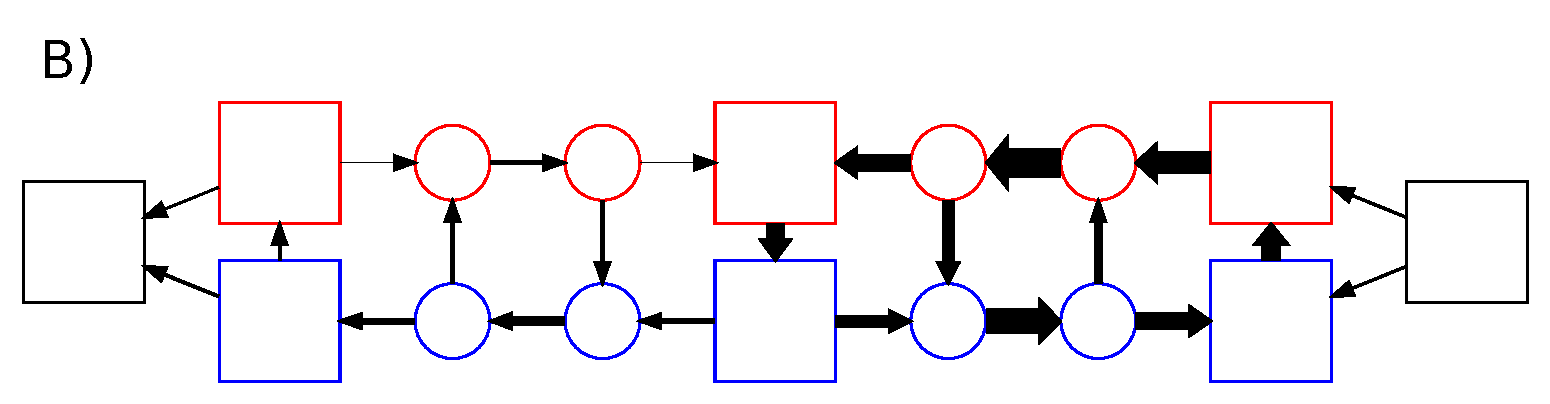
\includegraphics[width = 1 \textwidth]{plots/rep_flowchart1.pdf} 
        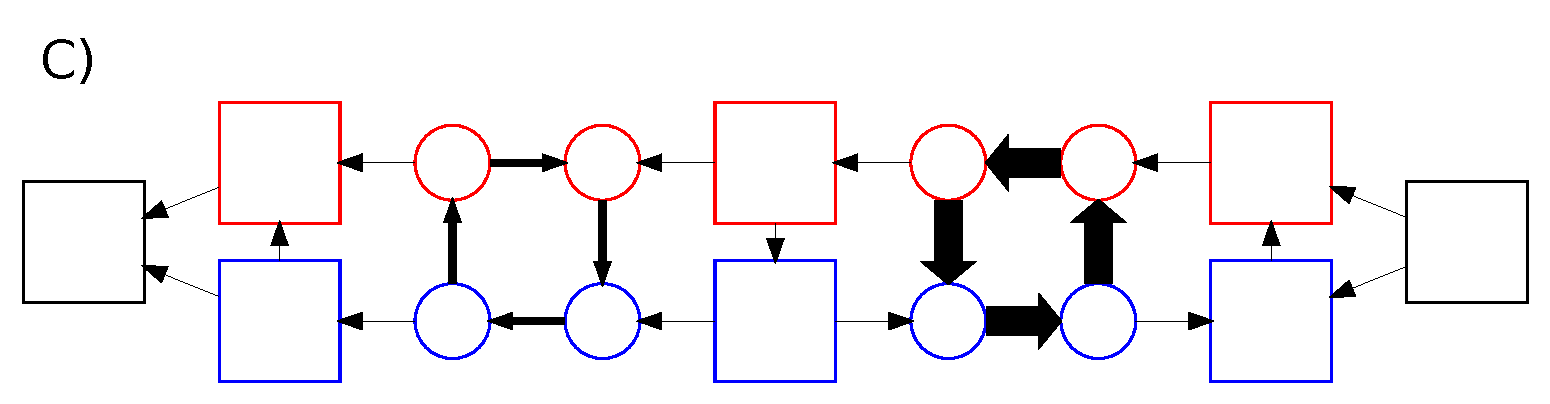
\includegraphics[width = 1 \textwidth]{plots/rep_flowchart2.pdf}
    \end{figure}
\end{minipage}
\vspace{0.5 cm} \\
It is obvious from this illustration that the system behaves qualitatively different depending on the decay length $r_d$.
\begin{itemize}
    \item For long decay length as in figure \ref{fig:flow_repulsive} A) it is visible from the very narrow arrows connecting red and blue icons that the particles in both states are independent in good approximation. Therefore inactive particles are not hindered by the barrier on their way from the bath to the sink whereas active particles have to overcome the potential barrier and are thus less likely to interact with the sink. Ether way, particles are very unlikely to change their state in the process. 
    \item For short decay length as in figure \ref{fig:flow_repulsive} C) the behavior is clearly different. Particle movement is closely tied to the potential boundaries at $r=a$ and $r=b$. There active particles are very likely to cross the boundary in downward direction only. Therefore the potential drives a spatial selection of particles that leads to an excess of active particles right outside and a deficit of active particles inside the barrier. The resulting difference in concentration of active and inactive particles at both sides of the barrier boundary leads to a strong reactive fluxes. Inside the barrier particles switch from inactive (red) to active (blue) and outside the barrier they switch from active to inactive state. The resulting imbalance of inactive particles draws them across the barrier from the out to the inside. As obvious from the flow diagram, the result is a strong \emph{circular current}. Since most of the particles switch states before they can diffuse more than $r_d$ away, the process is closely tied to the barrier boundaries. 
    \item For medium decay length as in figure \ref{fig:flow_repulsive} B) these circular currents are still existent but not so closely tied to the boundaries of the barrier. Therefore they overlap in space. This has the effect that once a particles has crossed the outer boundary of the barrier as part of one circular current it can switch to the other circular current to cross the inner boundary of the barrier. 
\end{itemize}
In the case of an attractive potential barrier the processes at work are quite similar. The differences to the repulsive case are outlined on the basis of the following flow diagrams: \vspace{-.5 cm} \\
\begin{minipage}[t]{.372 \textwidth}
    \vspace{.5 cm}
    \begin{figure}[H]
        \caption{Flow diagram for attractive barrier: This plot shows spatial and reactive particle flows between different particle species (active particles are represented in blue, inactive particles are represented in red) and different spatial regions (see figure \ref{fig:flowchart_scetch} for reference) for the examples given in figure \ref{asd}. The difference between the different plots is again the decay length which is equal to \newline A): $r_d=250$, B): $r_d=2.5$ and \newline C): $r_d = 0.25$.
    \label{fig:flow_attractive}}
    \end{figure}
\end{minipage}\hspace{0.02 \textwidth}\begin{minipage}[t]{.608 \textwidth}
    \begin{figure}[H]
        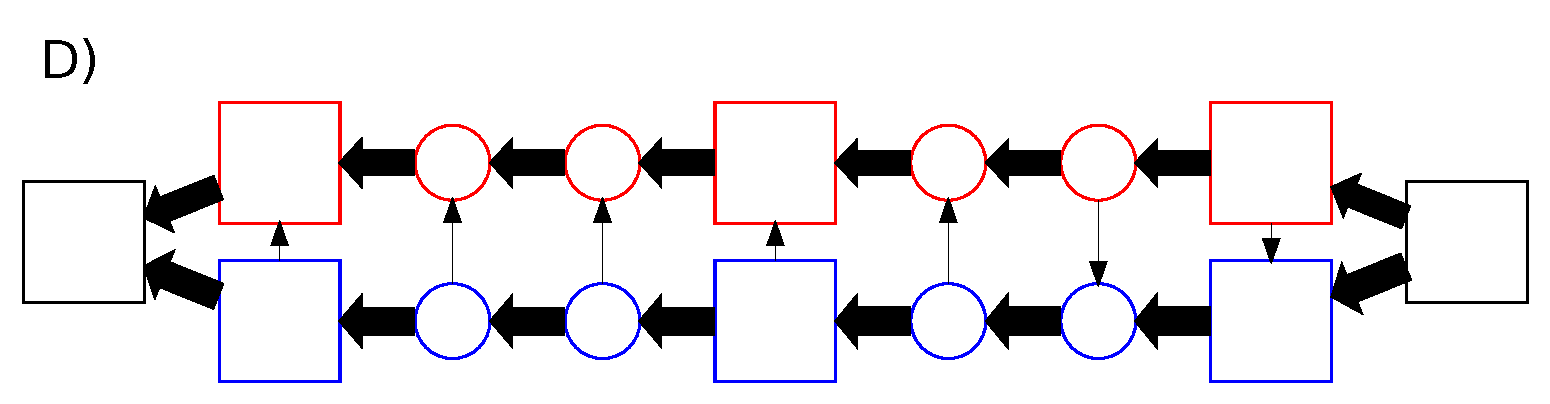
\includegraphics[width = 1 \textwidth]{plots/att_flowchart0.pdf}
        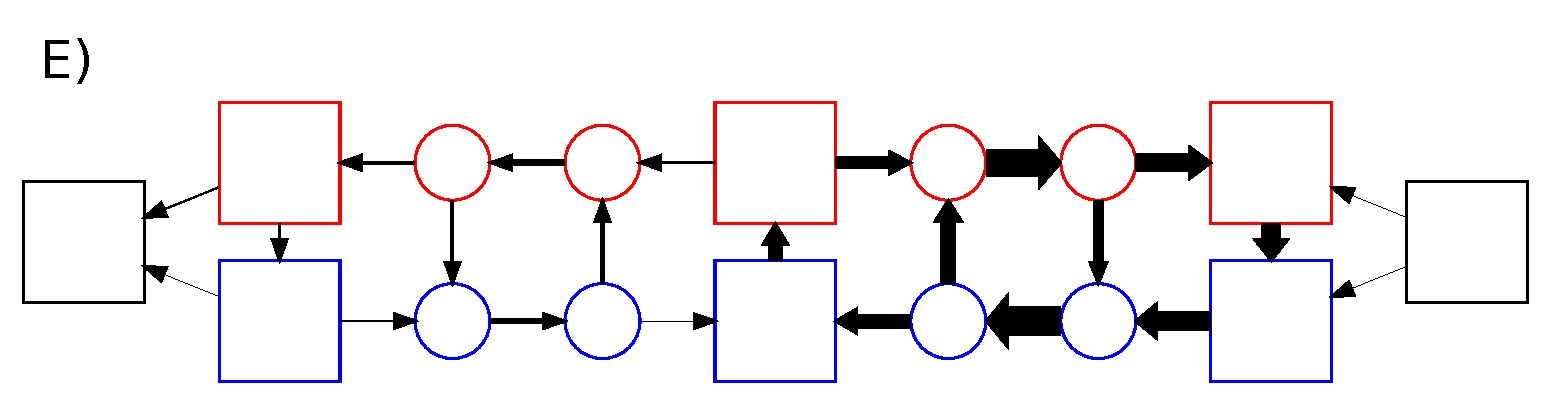
\includegraphics[width = 1 \textwidth]{plots/att_flowchart1.pdf}
        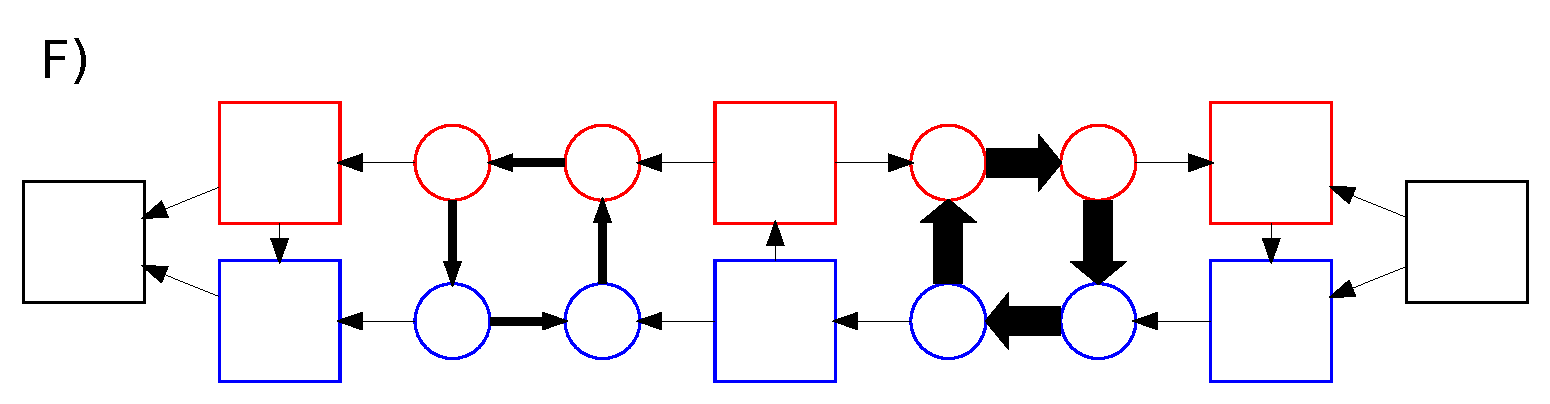
\includegraphics[width = 1 \textwidth]{plots/att_flowchart2.pdf}
    \end{figure}
\end{minipage}
\vspace{.5 cm} \\
The differences of these examples to the ones presented before in figure \ref{fig:flow_repulsive} can be pointed out one by one:
\begin{itemize}
    \item For long decay length as in figure \ref{fig:flow_attractive} D) the two particle species are independent from each other in good approximation. The difference to the former example is that the active particles are not hindered by the attractive barrier once the steady state is reached. They accumulate in the attractive potential until their concentration is high enough to to make it equally possible for particles to enter and leave the barrier (which is essentially given by the probability for particles to enter the potential). Therefore both particle species do equally contribute to the flux of particles from the bath to the sink.
    \item For short decay length as in figure \ref{fig:flow_attractive} F) the system again shows strong circular currents around the boundaries of the potential barrier. The difference is here that if active particles now cross the barrier in downward direction this means from the ``out'' to the ``in'' side. Therefore the circular currents are now directed in the other direction (clockwise vs. counter clockwise in this representation).
    \item For medium decay length as in figure \ref{fig:flow_attractive} E)  the two circular currents overlap just as they do in the case of a repulsive barrier. Therefore it is again likely for active particles to be drawn across the outer border of the potential by one current and then cross the boundary of the inner barrier as part of the other current.
\end{itemize}
This analysis has shown how the system behaves qualitatively different depending on the switching rate of the barrier $W$ or rather depending on the decay length $r_d$ of the particle densities. Knowing this, it is now time to turn to the key quantity in this investigation which is the reaction rate of particles interacting with the sink. 
\section{Absorption Rates}
Previously the focus was directed on the distribution of Brownian particles in the system. The distribution was explored for different magnitudes of the systems' decay length and qualitative differences were explained by the steady state flow of particles that emerged from the coupling of the barrier fluctuations to the diffusive particle movement.\\
The next section will explore the implications of these qualitative differences on the reaction rate of particles with the sink in the center of the system. This rate can be calculated from the density profiles via equation \eqref{Rate}. In the following the reaction rate is normalized to the Smoluchowski reaction rate $K_S$ \eqref{steady state ideal rate} for an ideal sink without any barrier . This way the influence of the potential barrier can be pointed out explicitly. \\
An analytic expression for the reaction rate is given in Appendix A.
Sadly, this form of the solution is longish, bulky and does not tell very much about the actual behavior of the reaction rate. Nevertheless, it can be used to plot the reaction rate in the case of the two examples that were studied so far: \\
\begin{minipage}[t]{0.5 \textwidth}
    \begin{figure}[H]
        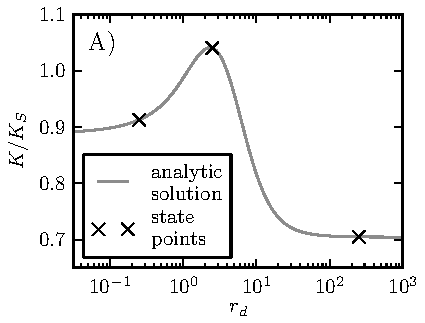
\includegraphics[width = 1 \textwidth]{plots/rb_rate.pdf}
    \end{figure}
\end{minipage}\begin{minipage}[t]{0.5 \textwidth}
    \begin{figure}[H]
        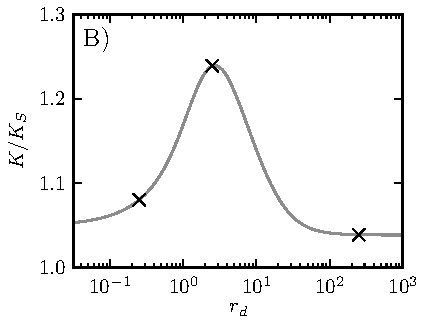
\includegraphics[width = 1 \textwidth]{plots/ab_rate.pdf}
    \end{figure}
\end{minipage}

\begin{minipage}[t]{1 \textwidth}
    \begin{figure}[H]
        \caption{Reaction rate of Brownian particles depending on the decay length of particle density for A) a repulsive barrier and B) an attractive barrier. The decay length and resulting reaction rate for the examples illustrated before are marked with black crosses. Those from figures \ref{rsd} and \ref{fig:flow_repulsive}  are marked in A), and those from figures \ref{asd} and \ref{fig:flow_attractive} are marked in B).\label{reaction_rate_examples}}
    \end{figure}
\end{minipage}
\vspace{.5 cm} \\
It is obvious from these plots that the reaction rate converges to finite values for very small and very large decay length and that it takes some maximum value in between. \\
Similar behavior has been studied for escape rates of Brownian particles trapped in fluctuating potentials. In this case the mean first passage time of the trapped particle over the barrier depends on the properties of the potential fluctuations. This has been extensively studied for different barrier shapes and different types of fluctuations \cite{Doering1992, Zurcher1993, Hanggi1994, Pechukas1994,Reimann1995a, Reimann1995}. \\
When Charles Doering and Jonathan Gouda first observed the phenomenon in 1992 \cite{Doering1992} they studied a particle that was trapped between a reflecting wall and a piecewise linear potential barrier that was subject to dichotomous Markovian noise. They observed that the mean first passage time of the particle over the barrier converged to finite values for very small and very long correlation times of the barrier fluctuations and exhibits a minimum in between. For this behavior they coined the term\textbf{ \emph{resonant activation}}.\\
Although this has only been studied for escape problems so far, the results presented here strongly suggest that it is also valid to use the term in the case of reaction rates over fluctuating barriers. \par
Even the underlying processes that have been studied in the previous section can be identified with those, that were found to be responsible for resonant activation in escape problems.
Referring to a first review paper on the topic published by Peter Reimann and Peter H\"anggi in 1997 \cite{Reimann1997} the case of a repulsive barrier can be identified with what they call ``Type I'' potentials, where particles enter the barrier region when it is in a low state and then get lifted up when the barrier switches to be subsequently able to escape. The case of an attractive barrier can be identified with what they call ``Type II'' or breathing barrier. In this case the part of the barrier that actually fluctuates is located right before the actual boundary that has to be overcome. The particle can enter the fluctuating area while it is in a low state, be then lifted when it changes to a high state and be subsequently able to cross the actual boundary. \par

Now, the next step in studying the vast expression that was derived for the reaction rate \eqref{two_state_rate} is evaluating some limits and trying to make sense of them in a physical way.
\section{Slow Fluctuation Limit}
\label{lim_long_rd}
For slow fluctuations of the potential barrier the decay length $r_d$ and therefore the spatial influence of the potential barrier becomes large compared to the length scale of the system. \\ 
To evaluate this limit, one uses equation \eqref{two_state_fpe} with symmetric rates, takes the limit of $W \rightarrow 0$ and considers the steady state case.
This results in two independent equations for the two particle species:
\begin{align}
    \frac{\partial \rho_1(r,t)}{\partial t} &= \vec \nabla \left[ D \vec \nabla \rho_1(r,t) \right], \\ \nonumber
    \frac{\partial \rho_2(r,t)}{\partial t} &= \vec \nabla \left[\rho_2(r,t) \vec \nabla \frac{U_2(r)}{\gamma} + D \vec \nabla \rho_2(r,t) \right]
    \label{two_state_fpe_W_to_0}
\end{align}
where $U_2$ has the form given in \eqref{step_potential}. \\
It is assumed that the detailed balance assumption and therefore the boundary condition for $r \rightarrow \infty$ remains valid despite the formal independence of the particle species.\\
The reaction rates for these independent equations can be calculated using the expressions given in \eqref{steady state ideal rate} and \eqref{K_Debye}. The combined rate can be derived as the weighted average of the two independent rates. Since the transition rates are taken to be symmetric, this results in:
\begin{align}
    K &= \frac{1}{2} \left[ 4 \pi D R_s^2 + 4 \pi D  \left\{\int_{R_s}^{\infty} \frac{\exp \left[ \frac{U_2(r')}{K_B T}\right]}{r'^2} \rm d r' \right\}^{-1} \right] \\ \nonumber
    &= 2 \pi D \left[ R_s^2 +\left\{\int_{R_s}^{a} \frac{1}{r'^2} \rm d r' + \int_{a}^{b} \frac{\exp \left[ \frac{U_2(r')}{K_B T}\right]}{r'^2} \rm d r' + \int_{b}^{\infty} \frac{1}{r'^2} \rm d r' \right\}^{-1} \right].
\end{align}
One evaluates the integrals, divides by the Smoluchowski reaction rate $K_S = 4 \pi D$, sets $R_s$ to one and substitutes $U_2/K_B T$ by $u$ to get:
\begin{align}
    \frac{K}{K_{S}} &= \frac{1}{2} \left[1 + \left\{ 1 -\frac{1}{a} + e^u \left(\frac{1}{a} - \frac{1}{b}  \right) + \frac{1}{b} \right\}^{-1} \right] \nonumber \\
    &= \frac{1}{2}\left[ 1 + \left\{ 1 + \left( \frac{1}{a} - \frac{1}{b} \right)\left( e^u -1 \right) \right\}^{-1} \right] \nonumber \\
    &= \frac{1}{2} \left[ 1 + \left\{ 1 - \frac{(b - a)}{ab}\left(1 - e^u \right) \right\}^{-1} \right] \nonumber \\
    &= \frac{1}{2} \left[ 1 + \frac{ab}{ab - \left( b-a \right)\left(1 - e^u \right)} \right].
    \label{two_state_K_slow}
\end{align}
The result of this somewhat intuitive calculation can then be compared to the slow switching limit of equation \eqref{two_state_rate}.
It proves to be sufficient to do a Taylor expansion around $\alpha_0 = 0$ to obtain
\begin{equation}
    \frac{K}{K_{S}} \approx \frac{(b-a)(1-e^u)-2ab }{2 \left((b-a) \left(1-e^u\right)-ab\right)} + \frac{  (b-a)^2\left(1-e^u\right)^2}{4 \left(ab + (b-a)(1-e^u)\right)^2} \alpha.
    \label{ksa}
\end{equation}
Where the leading term can be modified to take the form
\begin{equation}
    \lim_{\alpha \rightarrow 0} \frac{K}{K_{S}} =\frac{1}{2}\left(1+ \frac{ab}{ab-(b-a) \left(1-e^u\right)}\right).
    \label{klim0a}
\end{equation}
This is exactly the result, that was obtained in the previous calculation.
\section{Fast Fluctuation Limit}
\label{lim_short_rd}
For fast fluctuations of the potential barrier, there is another way to deal with equation \eqref{two_state_fpe}. In the limit of $W \rightarrow \infty$ the diffusion term can be neglected compared to the reactive terms, such that in the case of symmetric rates $\rho_1(r) \equiv \rho_2(r) = 2\rho(r)$ holds for all $r>R_s$. Therefore both equations can be added resulting in: 
\begin{equation}
    2 \frac{\partial \rho(r,t)}{\partial t} = \vec \nabla \left[\rho(r,t) \vec \nabla \frac{U_2(r)}{\gamma} + 2 D \vec \nabla \rho(r,t) \right].
    \label{fast_limit_fpe}
\end{equation} 
In other words this means that the timescale of the switching of particles between different states is much smaller than the timescale of spatial movement of the particles. As a result all particles move subject to a constant potential of mean force that is calculated as the weighted average of the potential in its different states. \\
Also, in the steady state case the time derivative of the density vanishes:
\begin{equation}
    0 = \vec \nabla \left[\rho(r,t) \vec \nabla \frac{U_2(r)}{2\gamma} + D \vec \nabla \rho(r,t) \right]
\end{equation}
such that the steady state rate can be calculated using the Debye formula \eqref{K_Debye}:
\begin{align}
    K &=  4 \pi D \left\{\int_{R_s}^{\infty} \frac{\exp \left[ \frac{U_2(r')}{2 K_B T}\right]}{r'^2} \rm d r' \right\}^{-1} \nonumber \\
    &= 4 \pi D \left\{\int_{R_s}^{a} \frac{1}{r'^2} \rm d r' + \int_{a}^{b} \frac{\exp \left[ \frac{U_2(r')}{2K_B T}\right]}{r'^2} \rm d r' + \int_{b}^{\infty} \frac{1}{r'^2} \rm d r' \right\}^{-1}.
    \label{mean_potential_rate}
\end{align}
The evaluation of the integrals, substitution of $U_2/K_B T$ with $u$ and the normalization by the Smoluchowski reaction rate $K_S$ from equation \eqref{steady state ideal rate} results in:
\begin{equation}
    \lim_{\alpha \rightarrow \infty} \frac{K}{K_S} = \frac{ab}{ab - (b-a)(1-e^{u/2})}.
    \label{K_fast_limit_1}
\end{equation}
A useful examination of the fast switching limit of equation \eqref{two_state_rate} requires a bit more work.
To find the behavior in the limit of $r_d \ll 1 $, i.e. $\alpha \gg 1$ one takes a closer look at the different exponents that occur in the numerator and denominator of equation \eqref{two_state_rate}. Namely:
\begin{align}
& e_1 = (3a+b)\alpha, \nonumber \\
& e_2 = (2+2b)\alpha, \nonumber \\
& e_3 = (2+a+b)\alpha, \nonumber \\
& e_4 = 4a\alpha, \nonumber \\
& e_5 = (2+2b)\alpha \quad \textrm{and} \nonumber \\
& e_6 = (2a+2b)\alpha.
\end{align}
Using the fact that $b > a > 1$ one finds that for $\alpha \gg 1$ the terms containing $e_6$ dominate all others. Therefore numerator and denominator can be reduced to
\begin{align*}
    F_1' =& ( 1 + a \alpha + e^u (-1 + 3 a \alpha)) (-1 + 3 b \alpha + e^u (1 + b \alpha))\\
    F_2' =& (-1 + (4 - 3 a + b) \alpha + (2 a - 2 b + 3 a b) \alpha^2 + e^{2 u} (-1 + (4 + a - 3 b) \alpha \\
          &+ 3 (a (-2 + b) + 2 b) \alpha^2) + 2 e^u (1 + (-4 + a + b) \alpha + (2 a - 2 b + 5 a b) \alpha^2)).
\end{align*}
If then only linear and quadratic terms in $\alpha$ are collected one receives an expression that turns out to be a reasonably good approximation of the fast switching behavior of the solution: 
\begin{align}
    \frac{K}{K_{S}} \approx &a \left(3 e^u+1\right) \left(e^u (b x+1)+3 b x-1\right)-b \left(2 e^u+e^{2 u}-3\right) / \nonumber \\
                          &\left\{a \left(e^{2 u} (3 (b-2) x+1)+2 e^u ((5 b+2) x+1)+3 b x+2 x-3\right) \right.  \nonumber \\
                          & \left. +\left(e^u-1\right) \left(b \left(3 e^u+1\right) (2 x-1)+4 \left(e^u-1\right)\right) \right\}
    \label{kla}
\end{align}
and in the actual limit of $\alpha \rightarrow \infty$ one obtains: 
\begin{equation}
    \lim_{\alpha \rightarrow \infty} \frac{K}{K_{S}} = \frac{a b \left(e^u+3\right)}{ab \left(e^u+3\right)-2(b-a)(1-e^u)}.
    \label{kliminfa}
\end{equation}
This can be simplified to 
\begin{align}
    \lim_{\alpha \rightarrow \infty} \frac{K}{K_S} &= \frac{ab}{ab - (b-a)(1-e^{u/2}) \kappa}, \\
    \kappa &= \frac{2(1+e^{u/2})}{e^u + 3}.
    \label{K_fast_limit_2}
\end{align}
This is clearly not equal to the limit that was obtained in equation \eqref{K_fast_limit_1}.\par
Now, lets see, if it is possible to understand this difference and to learn something from it. To do so it is useful to properly outline the differences in the derivation of these results.
Therefore it is crucial to realize that it is in fact \emph{two} limits that were taken in the process and that their order differed between the two calculations. One limit is that of the decay length $r_d \rightarrow 0$. The other limit concerns the spatial area of the change of the potential barrier, i.e. the width $r_F$ of the spherical shell in which the Brownian particles are actually subject to a force from the barrier. \\
\vspace{-.8 cm} \\
\begin{minipage}[t]{0.372 \textwidth}
    \begin{figure}[H]
        \caption{Simple sketch to point out the order of limits taken for the derivation of equation \eqref{K_fast_limit_1} and \eqref{K_fast_limit_2}. Both derivations uncouple the original equations to derive an expression for the fast switching limit of the reaction rate but the order of limits differs. \label{sketch_of_limits}}
    \end{figure}
\end{minipage}\hspace{0.01 \textwidth} \begin{minipage}[t]{.608 \textwidth}
\begin{figure}[H]
    \centering
    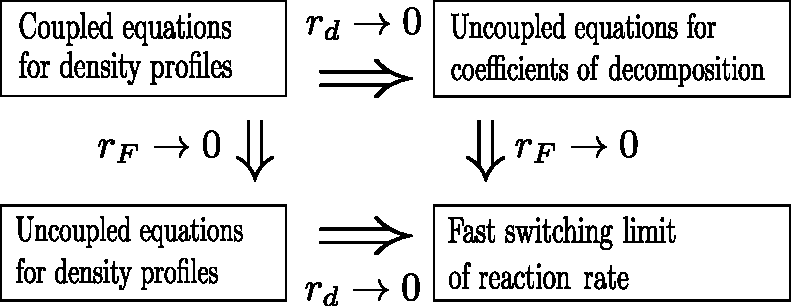
\includegraphics[width = 1 \textwidth]{plots/limits.pdf}
\end{figure}
\end{minipage}\par
Like it is illustrated in figure \ref{sketch_of_limits} the difference is the following: For the derivation of \eqref{K_fast_limit_1} the \emph{first} limit was that of $r_d \rightarrow 0$ and the \emph{second} limit was that of $r_F \rightarrow 0$ whereas for the derivation of \eqref{K_fast_limit_2} the \emph{first} limit was that of $r_F \rightarrow 0$ and the \emph{second} was that of $r_d \rightarrow 0$. \\
Since in general it is not equivalent to take limits in exchanged order it is not unexpected that the resulting expressions differ. The question is now: What does this mean in physical terms? \\

\newpage
\section{Numeric Study of Smooth Potential Barriers}
\label{Numeric_Study}
The easiest way to get an insight into the final question posed in the last section is to take a closer look at what actually happens, if the potential barrier does not vary in sharp jumps but does so on a finite length scale.
Therefore one examines how the reaction rate depends on the decay length of the particle density given a fixed but finite area on which the barrier changes. The natural way to do this is the application of a potential barrier that resembles a step function in shape and has a parameter to tweak this similarity. A generalized Gaussian:
\begin{equation}
    U_2(r) = U_2 \cdot \exp \left[ - \left( \frac{r_0 - r}{d} \right)^{2n} \right]
    \label{generalized_gaussian}
\end{equation}
with $r_0-d=a$ and $r_0+d=b$ serves this purpose well. The parameter $n$ can be used to control the width $r_F$ of the area of changes in the potential. It decreases as $n$ increases. \\
To compare the analytic results with numeric simulations they have to be derived with the same boundary conditions. Since it is not possible to set boundary conditions at infinity in numeric simulations one has to modify the boundary conditions \eqref{bcinf} in the analytic calculations. This can be done by setting 
\begin{equation}
    \vect{\rho}(R_m) = \vect{\rho}^{(eq)}
    \label{BC_for_numerics}
\end{equation}
where $R_m$ is the radius of the simulation domain. The numeric results for the reaction rate were derived by integrating the equations for the composite Markov process \eqref{two_state_fpe} using the method of lines described in section \ref{method_of_lines}. The results of this procedure are presented in the figure \ref{numeric}: \vspace{-0.5 cm}\\

The behavior that is observed in the comparison of numeric results with the analytic solution for the fluctuating step potential (FSP) \eqref{two_state_rate} and the rate over the static potential of mean force (PMF) \eqref{K_fast_limit_1} tells a couple of interesting things:
\begin{itemize}
    \item First, the resonant activation phenomenon that is observed for step potentials does also emerge for smooth potentials and is not an artefact or a mathematic curiosity. In fact the effect does get even stronger if the change of the potential happens on a finite length scale.
    \item Second, for $r_d \gg r_F$ the numeric results are well represented by the solution derived in \ref{Reaction_Rates_over_Fluctuating_Barriers} whereas for $r_d \ll r_F$ they show good agreement with the rate over a PMF. It is especially interesting, to have a closer look at the transition from the first to the latter case.
\end{itemize}
\begin{minipage}[t]{.5 \textwidth}
    \begin{figure}[H]
        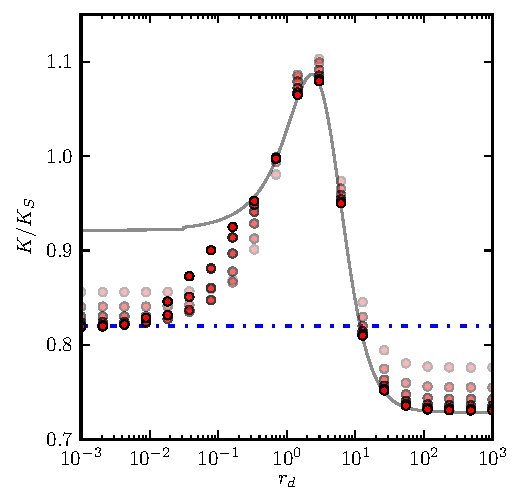
\includegraphics[width = 1 \textwidth]{plots/rb_cs.pdf}
    \end{figure}
\end{minipage}\begin{minipage}[t]{.5 \textwidth}
    \begin{figure}[H]
        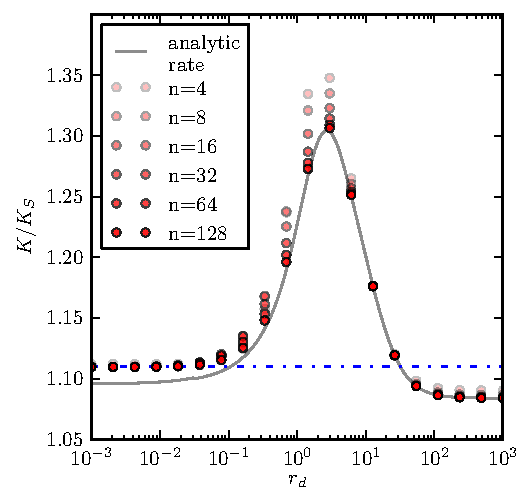
\includegraphics[width = 1 \textwidth]{plots/ab_cs.pdf}
    \end{figure}
\end{minipage}

\begin{minipage}[t]{1 \textwidth}
    \begin{figure}[H]
        \caption{Comparison of numeric and analytic results for repulsive (\emph{left}) and attractive (\emph{right}) fluctuating barrier. The numeric results are obtained via the method of lines \ref{method_of_lines}. The reaction rate over the potential of mean force \eqref{K_fast_limit_1} is indicated by the dashed blue line. The analytic solution over the fluctuating step shaped barrier in equation \eqref{two_state_rate} is indicated by a solid grey line. The radius of the simulation domain is $R_m=30 R_s$. The other parameters are the same as in the previous examples and given in \ref{Parameters}. The analytic solution represents the numeric results very well for large $r_d$ and small $r_F$. The numeric results converge away from the analytic solution for the step shaped fluctuating barrier and towards the rate over the potential of mean force for small $r_d$. Note that the smaller $r_F$ (large $n$) of the potential, the smaller the $r_d$ at which the transition takes place.\label{numeric}}
    \end{figure}
\end{minipage} \vspace{0.5 cm} \\

As it can be seen especially for the case of the repulsive barrier, the transition of numeric results from the description by a FSP to a PMF takes place at a different decay length for different spatial extend of the changes of the potential barrier.  The smaller the spatial extent of the changes $r_F$, the smaller the decay length $r_d$ at which the transition takes place. \\
One possible explanation for this can be given in terms of particle fluxes: In the case of the FSP one has $r_F=0$ and therefore the total reactive flux in the region of potential change vanishes. In the case of the PMF it is assumed that the reactive fluxes are strong enough to make both particle species have the same spatial distribution. In other words: In the case of a FSP the area of potential change is dominated by spatial fluxes whereas in the case of a PMF it is dominated by reactive fluxes.\\
Another possible explanation can be given in terms of times: In the case of the FSP the decay time $\tau_R = W/2$ of the state of a particle is much larger than the time $\tau_S$ that it takes for a particle to cross the area of potential change (since the area is actually of zero spatial extent). In the case of the PMF it is the other way around (since the inverse of the switching rate goes to zero). For a derivation of the decay time $\tau$ please refer to Appendix A.\\
The neat thing about these two ways of explaining the situation is that they are essentially the same and that they both give  an estimate for the parameter range in which eater the FSP or the PMF description is valid, and consequently where the transition from one to the other takes place.
For the PMF [FSP] the reactive flux and the spatial flux driven by the potential $J^{(R)}$ and $J^{(F)}$ in the region of potential change fulfill the following relation:
\begin{equation}
    J^{(F)} \ll[\gg] J^{(R)}.
\end{equation}
If the change of the potential is assumed to take place at a radius $r_0$ the according sphere surface $A$ and the volume of the potential change $V$ can be assumed to be roughly $A=4 \pi r_0^2$ and $V=4 \pi r_0^2\cdot r_F$. With this the previous expression reads:
\begin{equation}
    \frac{\rho(r_0)}{\gamma}\frac{{\rm d}U(r_0)}{{\rm d}r} A \ll[\gg]\rho(r_0) W V.
\end{equation}
    Since in the overdamped limit the mean velocity of a particle is given by $\bar{v}(r) = f(r)/\gamma$ this can be written as:
\begin{align}
    \frac{\bar{v}}{r_F} & \ll[\gg] W \nonumber \\
    \frac{1}{\tau_S} & \ll[\gg] \frac{2}{\tau_R}.
\end{align}
Which is the equivalence of the flux and the traveling resp. reaction time argument that was to be shown.
Both arguments give an estimation to when one or the other description is a valid approximation to calculate the reaction rate:
\begin{equation}
    \frac{\Delta U}{K_B T} \ll[\gg] \frac{r_F}{2 r_d}
    \label{val_estimate}
\end{equation}
This last result gives the parameter ranges in which the FSP [PMF] description is valid and shows that the decay length at which the transition between both descriptions takes place is defined by the hight of the potential barrier and the width of the area of its boundary.
\section{Summary}
In the previous section a simple example of reaction rates over a fluctuating barrier revealed some interesting effects. It turned out that resonant activation as previously seen with escape problems does also appear in reaction rates over fluctuating barriers. The effect was explained by an analysis of spatial and reactive particle fluxes and validated by numeric results. At the analysis of the fast switching limit it became obvious that the solution for the fluctuating step potential does inherently not reproduce the natural result of an effective potential of mean force. As a result of the analysis of this ambiguity an estimate for the validity of both descriptions was derived.

\newpage
\section{Influence of Barrier Spacing}
Until now, the boundaries of the potential barrier were fixed to $a=6 R_s$ and $b=11R_s$ and the main focus was directed on the influence of the decay length $r_d$. Since this is understood quite well now, the next section will have a closer look on the impact of the barrier spacing.\\
The barrier spacing is reasonably described by two free parameters. First, the ratio of the gap between barrier and the sink and the width of the barrier $g$ and second, its overall length scale $l$ relative to the radius of the Sink $R_s$:
\begin{equation}
    \frac{a}{R_s} - 1 = l, \qquad \frac{b-a}{R_s} = g \cdot l
    \label{spacing_variables}
\end{equation}
With these the relative and the overall spacing of the barrier can be varied independently. 
It would be interesting to know how these parameters influence the decay length that maximizes the reaction rate. Unfortunately the expression for the reaction rate \eqref{two_state_rate} is such, that its discussion leads to transcendental equations that can not be solved analytically. Therefore the influence of the barrier spacing and the barrier gap to width ratio can only be investigated qualitatively and numerically. Next the influence of the barrier gap to width ratio $g$ will be examined first. \\

\begin{minipage}[t]{.5 \textwidth}
    \begin{figure}[H]
        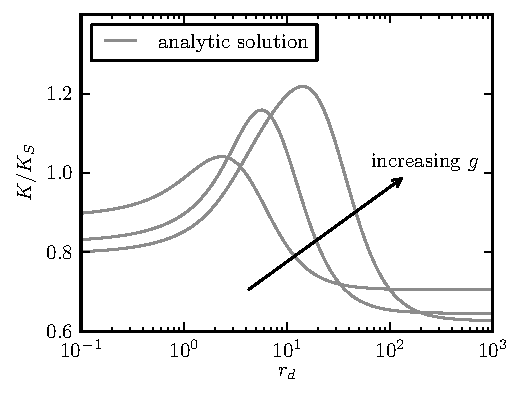
\includegraphics[width = 1 \textwidth]{plots/g2_rb_rates.pdf}
    \end{figure}
\end{minipage}\begin{minipage}[t]{.5 \textwidth}
    \begin{figure}[H]
        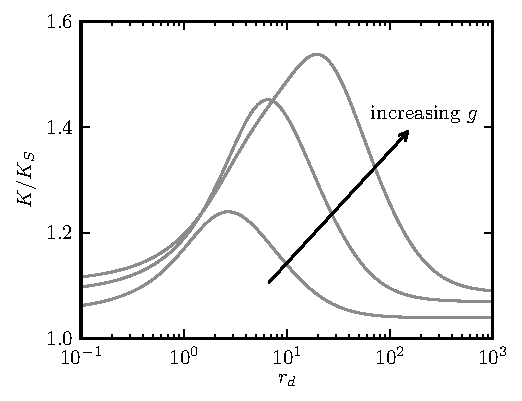
\includegraphics[width = 1 \textwidth]{plots/g2_ab_rates.pdf}
    \end{figure}
\end{minipage}

\begin{minipage}[t]{1 \textwidth}
    \begin{figure}[H]
        \caption{Reaction rates for different barrier gap to width ratio $g = 1, 4 ,16$ for repulsive fluctuating barrier (\emph{left}) and attractive (\emph{right}) fluctuating barrier. The overall barrier length scale $l$ is equal to $l=1 R_s$. The other parameters are given in \ref{Parameters}. It is obvious that the resonant activation effect also becomes more pronounced as the relative barrier width increases.\label{fig:var_g}}
    \end{figure}
\end{minipage} \vspace{0.5 cm} \\

The plots in figure \ref{fig:var_g} show, that influence of the barrier gap to width ratio $g$ is qualitatively different than that of the overall barrier spacing $l$. In the case of a repulsive barrier the reaction rates in the long and short decay length limits decrease if $g$ increases where it increased when $l$ increased. In the case of an attractive barrier the reaction rate in the long and short decay length limits increase if $g$ increases where it decreased when $l$ increased.
In both cases an increase in the gap to width ratio $g$ increases the decay length that maximizes the reaction rate and the resulting maximum reaction rate. Especially in the case of an attractive barrier it is obvious that the range of decay lengths that significantly increase the reaction rate becomes wider if $g$ increases. \\

The impact of the overall barrier spacing $l$ on the reaction rate is studied next.

\vspace{-0.5 cm}
\begin{minipage}[t]{.5 \textwidth}
    \begin{figure}[H]
        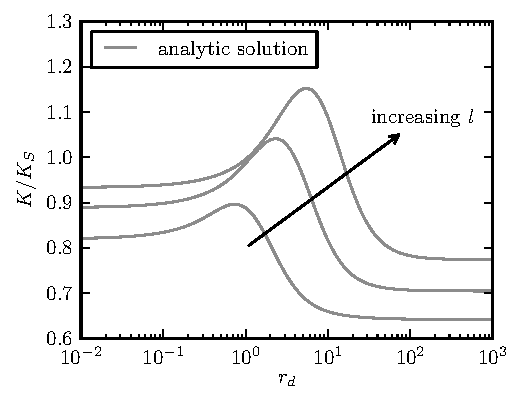
\includegraphics[width = 1 \textwidth]{plots/l2_rb_rates.pdf}
    \end{figure}
\end{minipage}\begin{minipage}[t]{.5 \textwidth}
    \begin{figure}[H]
        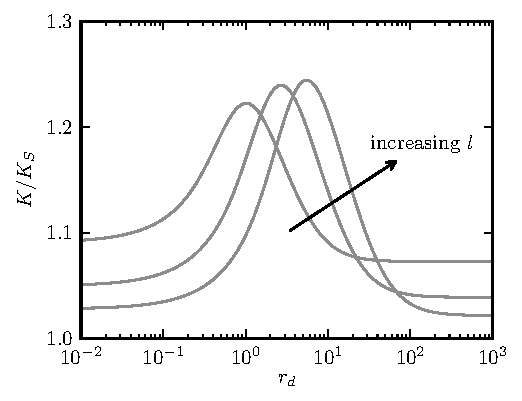
\includegraphics[width = 1 \textwidth]{plots/l2_ab_rates.pdf}
    \end{figure}
\end{minipage}\\
\begin{minipage}[t]{1 \textwidth}
    \begin{figure}[H]
        \caption{Reaction rates for different barrier spacing $l = 2 R_s, 5 R_s ,10 R_s$ for repulsive fluctuating barrier (\emph{left}) and attractive fluctuating barrier (\emph{right}). The ratio of the barrier width and the gap between sink and barrier $g$ is equal to one. The other parameters are given in table \ref{Parameters}. It is obvious that the resonant activation effect becomes more pronounced as the barrier spacing increases.\label{fig:var_l}}
    \end{figure}
\end{minipage} \vspace{0.5 cm} \\
The plots in figure \ref{fig:var_l} show that the barrier spacing has different impact on the long and short decay length limits of the reaction rate for in case of an attractive or repulsive barrier.
In the case of a repulsive barrier a larger barrier spacing increases the reaction rate in the short and long decay length limits. In the case of an attractive barrier a larger barrier spacing decreases the reaction rate in the short in long decay length limits. In both cases the decay length that maximizes the reaction rate as well as the resulting maximum reaction rate increase with a larger barrier spacing. The increase in the maximum reaction rate is stronger when the barrier is repulsive.\\
Further investigation of the dependence of the maximum reaction rate on the barrier spacing can be done numerically. Therefore one evaluates the roots of the first derivative of the analytic expression of the reaction rate given in equation \eqref{two_state_rate}. \\
\vspace{-0.5 cm}
\begin{minipage}[t]{.5 \textwidth}
    \begin{figure}[H]
        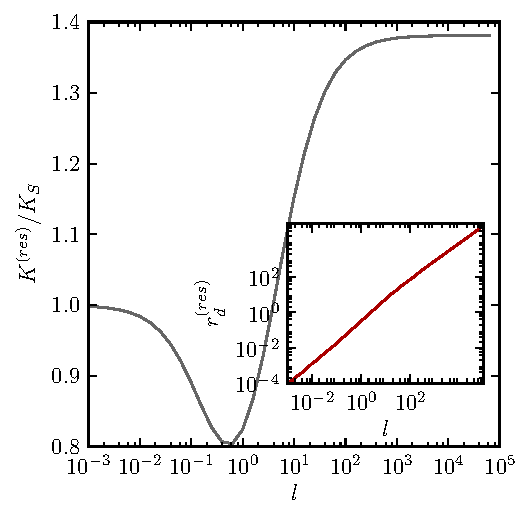
\includegraphics[width = 1 \textwidth]{plots/rep_l.pdf}
    \end{figure}
\end{minipage}\begin{minipage}[t]{.5 \textwidth}
    \begin{figure}[H]
        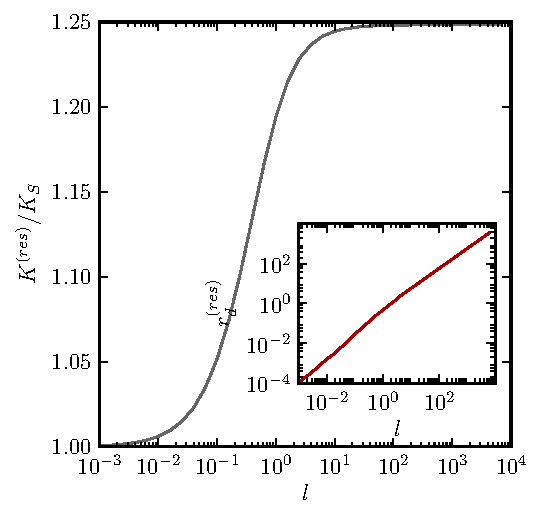
\includegraphics[width = 1 \textwidth]{plots/att_l.pdf}
    \end{figure}
\end{minipage}\\
\begin{minipage}[t]{1 \textwidth}
    \begin{figure}[H]
        \caption{Numeric evaluation of the maximum reaction rate $K^{(res)}$ depending on barrier spacing $l$ for repulsive fluctuating barrier (\emph{left}) and attractive fluctuating barrier (\emph{right}). The subplot gives the decay length $r^{(res)}$ that maximizes the reaction rate for each given barrier spacing $l$. The ratio of the barrier width and the gap between sink and barrier $g$ is equal to one. The other parameters are given in table \ref{Parameters}. It is obvious that the maximum reaction rate saturates for very large barrier spacing and that it becomes equal to the Smoluchowski reaction rate $K_S$ for a sink without barrier for very small barrier spacing. \label{fig:res_l}}
    \end{figure}
\end{minipage} \vspace{0.5 cm} \\

It is obvious from the plots in figure \ref{fig:res_l} that the maximum reaction rate for both, the attractive and the repulsive fluctuating barrier converge to the Smoluchowski reaction rate \eqref{steady state ideal rate} if the barrier spacing $l$ goes to zero. For very large barrier spacing the reaction rate converges to a finite value in both cases. \\
For the attractive fluctuating barrier the maximum reaction rate interpolates monotonously between these two values. For the repulsive fluctuating barrier the reaction rate has a local minimum. A possible explanation for this is, that for very small $l$ the barrier has no influence at all (this is in fact the case for barriers of finite hight, as will be shown in the following sections). For small but finite barrier spacing the barrier is mainly hindering particles from crossing and contacting the sink and only for larger barrier spacing the effect of overlaying circular currents illustrated in figure \ref{fig:flow_repulsive} of section \ref{flow_analysis} becomes stronger than the inherent shielding effect of the barrier.\\
Note that for large $l$ this can lead to reaction rates that are significantly (up to 40 \%) higher than than the reaction rate without a barrier and also higher than the highest possible reaction rate over a fluctuating attractive barrier.\\
So if this effect can be found in experiments where one usually only observes time averaged parameters such as the potential of mean force of the barrier and the reaction rate this must look confusing. The rate over the repulsive potential is notably higher than the rate over the attractive potential although classical Debye rate theory as outlined in \ref{The_Debye_Reaction_Rate} suggests the opposite.

\section{Influence of the Barrier Height}
This section investigates the influence of the barrier hight on the reaction rate. It gives the limiting behavior of the system for an infinitely attractive and an infinitely repulsive barrier and outlines the behavior for intermediate barrier heights.\\
Analytic expressions for the limits can be derived analytically from the formula for the reaction rate \eqref{two_state_rate}. The resulting expressions \eqref{attractive_limit} and \eqref{repulsive_limit} are given in Appendix B.

\begin{minipage}[t]{.64 \textwidth}
\begin{figure}[H]
    \centering
    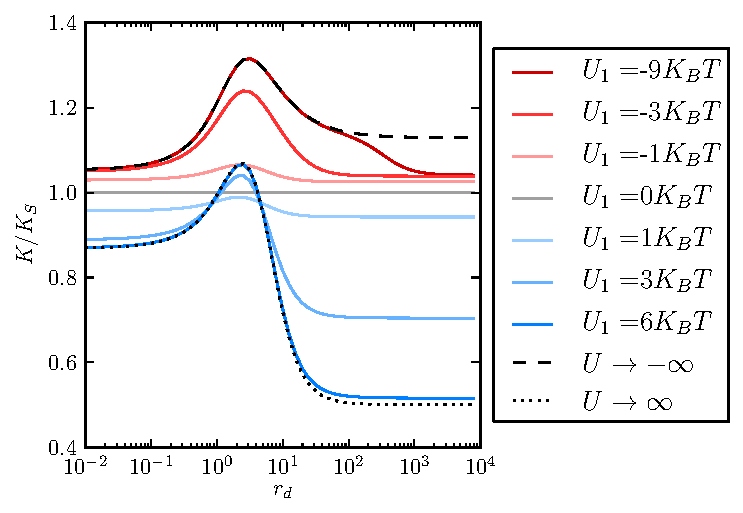
\includegraphics[width = 1 \textwidth]{plots/u1_dependence}
\end{figure}
\end{minipage} \hspace{0.01 \textwidth} \begin{minipage}[t]{.35 \textwidth}
    \begin{figure}[H]
        \caption{Adsorption rate vs decay length for various barrier heights $U_1$. The analytic limits for an infinitely attractive barrier \eqref{attractive_limit} and an infinitely repulsive barrier \eqref{repulsive_limit} are given by dashed and dotted black lines respectively. The barrier spacing in terms of $a$ and $b$ is given in \ref{Parameters}. \label{u1_dependence}}
    \end{figure}
\end{minipage}

Figure \ref{u1_dependence} shows the reaction rate normalized to the Smoluchowski reaction rate $K_S$ as a function of the decay length $r_d$ for different barrier heights $U_1$ as well as the limits for $U_1 \rightarrow -\infty$ of a perfectly attractive barrier and the limit of $U_1 \rightarrow \infty$ of a perfectly repulsive barrier.
It is obvious that for vanishing barrier hight the rate is equal to the ideal Smoluchowski rate \eqref{steady state ideal rate} as one would expect. For an attractive barrier the reaction rate monotonously interpolates between the ideal Smoluchowski rate and the limit of an ideal attractive barrier. For a repulsive barrier the reaction rate monotonously interpolates between the ideal Smoluchowski rate and the limit of an ideal repulsive barrier only for small and large decay lengths. For decay lengths around the resonant decay length the reaction rate first decreases for small $|U_1|$ and then increases to values above the ideal Smoluchowski rate. This is somewhat similar to the dependence of the rate on the barrier spacing observed in \ref{fig:res_l} where for small barrier spacing the resonant reaction rate first decreased below and then increased above the ideal Smoluchowski rate for increasing barrier spacing. \par
One more effect is visible in figure \ref{u1_dependence} that emerges for strongly attractive barriers. The fast switching limit of finitely and infinitely attractive barriers is obviously not equal as the fast switching limit is significantly higher for the infinitely attractive barrier. It is also visible, that for higher $|U_1|$ the reaction rate is similar to the $U_1 \rightarrow -\infty$ limit up to higher decay lengths. To understand this effect reconsider the assumption that has been made in section \ref{lim_long_rd} to derive the slow switching/hight decay length limit of the reaction rate. Here one assumed that for sufficiently slow barrier switching the two states of the barrier can be treated independently. This also implies, that the transient time, that is necessary for the particle density to equilibrate after a barrier switch is small compared to the decay time of the state of the barrier. As it turns out the timescales cannot be separated for diverging $|U_1|$ if the barrier is attractive.\\
The explanation of the effect is most intuitive, if the fluctuations are taken to be a property of the barrier. For an illustration of the density profiles in the slow switching limit for an attractive barrier please refer to figure \ref{asd} A). \\
In its active state the attractive barrier acts as a reservoir that collects particles until the density in the area of the barrier is high enough that the probability of particles to leave the barrier is equal to the probability of particles to enter the barrier. According to the fit conditions derived in \ref{Fit_Conditions} this is given if the quotient of the densities at the sink boundary is equal to the Arrhenius factor $\exp[-U_1/K_B T]$. Also for long times the adsorption rate to the boundary is limited by the ideal Smoluchowski rate to a sink with radius equal to the radius of the outer barrier boundary. Consequently the time for the equilibration of the density profile scales exponentially with the barrier hight and therefore the timescales of density relaxation and barrier fluctuation can not be decoupled, if $U_1$ goes to infinity. For large but finite $U_1$ the reservoir effect of the attractive barrier leads to an increase of the reaction rate even for very slow barrier switching.
\newpage
\section{The one dimensional Limit}
After what has been observed in the previous two sections concerning the influence of barrier spacing and barrier hight, there is one more interesting limit to take which is the limit of $l \rightarrow 0$ i.e. that of an infinitely narrow barrier. This limit is interesting for two reasons. \\
First, it reveals the influence of the barrier curvature. As depicted in figure \ref{fig:llimit_skizze} for very small barrier spacing the system locally looks like a fluctuating barrier in front of an absorbing wall that is supplied with a constant influx of particles from infinity. So, the limit of $l \rightarrow 0$ should show effects that persist even without curvature and in leading order and should give curvature dependent effects in higher orders of $l$.\\
Second, it bridges the gap to the problem of a gated sphere, since for infinitely small barrier spacing and infinite barrier hight the system is equivalent to a sphere, that fluctuates between a state of an absorbing and a state of a reflecting surface.
\\ \vspace{-1 cm}

\begin{minipage}[t]{.372 \textwidth}
    \vspace{0.5 cm}
    \begin{figure}[H]
        \caption{Sketch for the limit of $l\rightarrow 0$. If the spacing of the barrier becomes small relative to the radius of the sink, then also the local curvature of the system vanishes i.e. for a particle that is located in the vicinity of the barrier the system looks like a fluctuating barrier in front of an absorbing wall. Therefore, in this limit the system spatially reduces to one dimension.
    \label{fig:llimit_skizze}}
    \end{figure}
\end{minipage}\hspace{0.04 \textwidth}\begin{minipage}[t]{.608 \textwidth}
    \begin{figure}[H]
        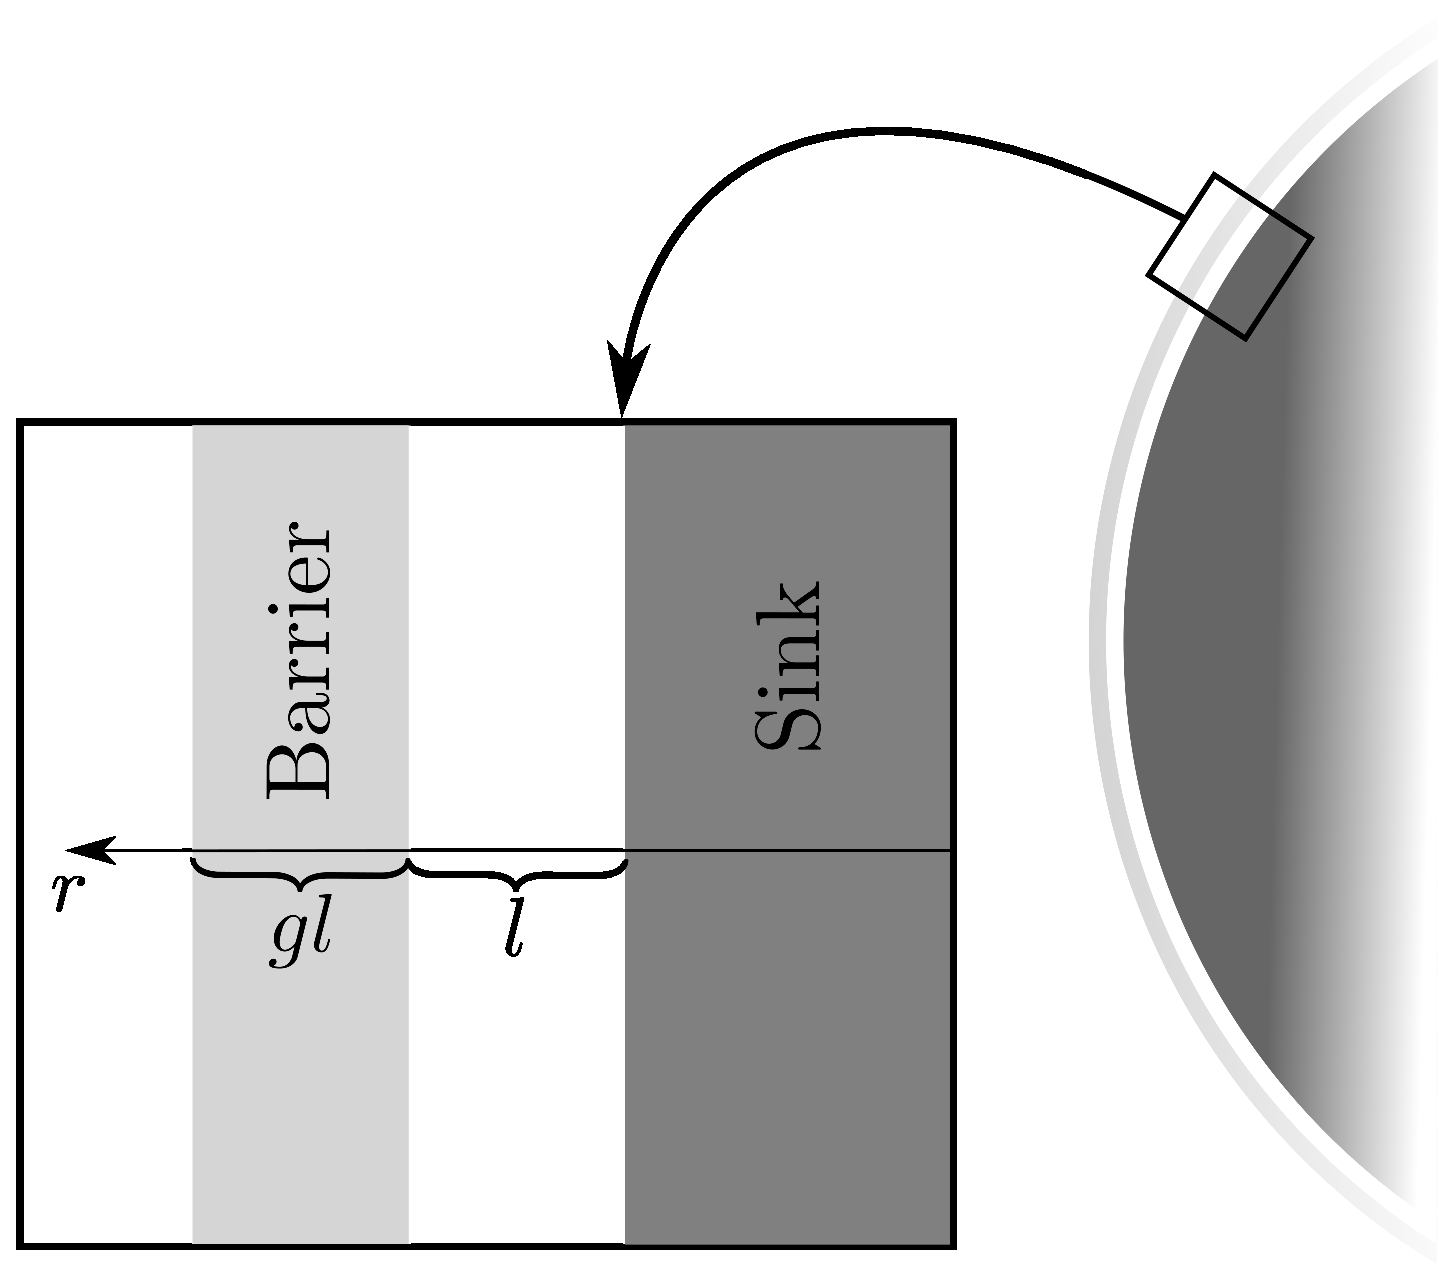
\includegraphics[width = 1 \textwidth]{plots/tlimit.eps}
    \end{figure}
\end{minipage}
\vspace{0.5 cm} \\
The limit is taken for three different situations. For an infinitely attractive barrier, for an infinitely repulsive barrier and for a barrier of finite hight. Therefore the appropriate expressions for the reaction rate \eqref{two_state_rate}, \eqref{attractive_limit} and \eqref{repulsive_limit} are used as a starting point. For each of these expressions one does a Taylor expansion around $l=0$ to obtain the following results:
\begin{itemize}
    \item for a barrier of finite hight:
\end{itemize}
\begin{equation}
    \frac{K}{K_S} \approx 1 + \frac{1}{2}\left(1- \exp\left[\frac{U_1}{K_B T}\right]\right)gl + \mathcal{O}(l^{2}),
    \label{llim_finite}
\end{equation}
\newpage
\begin{itemize}
    \item for an infinitely attractive barrier:
\end{itemize}
\begin{equation}
    \frac{K}{K_S} \approx 1 + \frac{gl}{4} + \mathcal{O}(l^{2}),
    \label{llim_att}
\end{equation}
\begin{itemize}
    \item and for an infinitely repulsive barrier:
\end{itemize}
\begin{equation}
    \frac{K}{K_S} \approx \frac{1+r_d}{1 + 2 r_d} - \frac{(g+1)l}{(2r_d+1)^{2}} + \mathcal{O}(l^{2}).
    \label{llim_rep}
\end{equation}

What is striking is that for the finite and the infinitely attractive barrier the leading order of the reaction rate is simply one. It does nether depend on the barrier hight, nor on the barrier gap to width ratio $g$. And even the fist correction does not depend on the barrier fluctuations. This means, that in the one dimensional limit the fluctuations of the barrier do not have any effect. Consequently, the curvature of the barrier must be crucial for any resonance effects to arise.\\
Concerning the gated sphere one could suspect, that a barrier of finite hight and infinitely small spacing would result in a non ideal sink, i.e. one that does not absorb every particle that comes in contact with its surface since it would have to overcome the barrier first, in which it would succeed only with a probability proportionate to an Arrhenius factor $\exp\left[U_1/K_B T \right]$. As it turns out, this is not the case. To show this, one uses the expression for the Debye reaction rate \eqref{K_Debye} and calculated is for a step shaped potential of hight $U_1$ with boundaries at $1+l$ and $1+l+lg$.
\begin{align}
    K_D   &= 4 \pi D \rho_0 \left\{ \int_{1}^{\infty} \frac{\exp \left[U(r)/K_B T \right]}{r^2} {\rm d} r \right\}^{-1} \nonumber \\
    &=4 \pi D \rho_0 \left\{ \int_{1}^{1+l} \frac{1}{r^2}{\rm d}r + \int_{1+l}^{1+l+lg} \frac{\exp \left[U_1/K_B T \right]}{r^2} {\rm d} r + \int_{1+l+lg}^{\infty}\frac{1}{r^2}{\rm d}r \right\}^{-1} \nonumber \\
    &= 4 \pi D \rho_0 \left\{ \frac{1}{1+l} + \frac{1}{1+l+lg} + \frac{g l}{ (1+l)(1+l+lg)} \right\}^{-1}
    \label{Debye_llimit}
\end{align}
This expression is normalized to the Smoluchowski rate $K_S$ \eqref{steady state ideal rate} and Taylor expanded around $l=0$:
\begin{equation}
    K_D \approx 1+\left(1-\exp\left[\frac{U_1}{K_B T}\right] \right)gl + \mathcal{O}(l^2).
    \label{Debye_taylor}
\end{equation}
It is obvious, that up to linear order in $l$ the small spacing limit of the reaction rate over the fluctuating barrier \eqref{llim_finite} is equal to the average of the Debye rate over the step shaped barrier and the Smoluchowski rate for an ideal barrier. \\
Again, the leading term is equal to one, i.e. for vanishing barrier spacing the barrier has no influence on the adsorption rate. Consequently, the connection to gating can only be made for an infinitely hight fluctuating barrier i.e. in the case when the barrier is assumed to be infinitely hight first before the expansion in $l$ is done (the order of the limit matters, as already noted in section \ref{lim_short_rd}). \\
Indeed, the case of the ideal repulsive barrier \eqref{llim_rep} is the only one, where the reaction rate depends on the barrier fluctuations in the leading order term. The reaction rate interpolated monotonously between $K/K_S = 1$ for $r_d = 0$ and $K/K_S = 0.5$ for $r_d \rightarrow \infty$. These limits are in agreement to what has previously been found for the problem of a gated sphere by Szabo et al. \cite{Szabo1982}. 
They studied the problem of a gated sphere that switches between a first state where its surface reflects incoming particles and a second state where it absorbed incoming particles with a certain surface reaction rate. The called this process opening and closing of the gate.
They found that 
\begin{itemize}
    \item given diffusive relaxation is slow compared to the opening and closing of the gate, the reaction rate is equal to the adsorption rate that would be observed without gating times the probability that the gate is open and
    \item given that the diffusive relaxation is fast compared to the opening and closing of the gate, the spherical sink behaved as if its gate was always open.
\end{itemize}
Since in the case under study the Sink is taken to be ideal, the surface reaction rate of the sink is infinite and the adsorption rate without a barrier is equal to the ideal Smoluchowski rate \eqref{steady state ideal rate}. Also the barrier fluctuations are taken to be symmetric, such that the probability for the barrier to be in one of its two states is equal to one half.
Consequently the findings of Szabo et al. translate to:
\begin{itemize}
    \item slow diffusion relaxation compared to the barrier switching (gating) is equivalent to large $r_d$ where the adsorption rate for the infinitely repulsive barrier of infinitely small spacing is equal to half of the ideal Smoluchowski rate, that would be observed without the barrier,
    \item fast diffusive relaxation and compared to the barrier switching is equivalent to small $r_d$ where the adsorption rate for the infinitely repulsive barrier of infinitely small spacing is equal to the Smoluchowski rate, i.e. it behaves as if the barrier was not there.
\end{itemize}


\newpage
\section{Mapping on a Non-Markovian Description}
\subsection{Common Assumptions}
When an experimentalist would investigate on a realization of the system under study in this thesis he would probably proceed as Shuan Wu et al. \cite{Wu2012a} and do the following: \\ 
He would \emph{first} assume a potential of mean force $U_m(r)$ for the barrier and then calculate the reaction rate using Debye rate theory with a spatially depending diffusivity profile $D(r)$:
\begin{equation}
    K_D^{-1} = \int_{R_s}^{\infty}\frac{\exp[U_m(r)/K_B T]}{4 \pi r^{2} D(r)} {\rm d} r.
    \label{YSDebye}
\end{equation}
and \emph{second}, if the adsorption to the sink in the system would not be ideal but subject to some surface reaction rate $K_S$ he would assume the diffusion controlled and the surface reaction part to independent and calculate the effective reaction rate as:
\begin{equation}
    K_{eff}^{-1} = K_D^{-1} + K_S^{-1}.
    \label{Keff}
\end{equation}
There is a list of problems with these two assumptions that will be outlined in the following discussion. \\
\subsection{First Assumption}
As was shown in section \ref{Numeric_Study} the description of the rate by Debye theory is only valid for smooth potentials and for these only if the switching of the potential is much faster that the diffusion of the Brownian particles. Otherwise both processes couple and the assumption is violated. Moreover, if one sticks to Debye theory and uses the particle density which might be measured and the potential of mean force to calculate an effective spatial diffusivity profile $D_{eff}(r)$ from: 
\begin{equation}
    \rho_D = C \exp\left[\frac{-U_m(r)}{K_B T}\right] \int_{R_s}^{r} \frac{\exp\left[\frac{U_m(r')}{K_B T}\right]}{4 \pi r'^{2} D_{eff}(r)}{\rm d} r'
    \label{Deff}
\end{equation}
this will lead to artificial results. To picture this, one uses two different methods to calculate an effective diffusivity profile. First one uses the Method of Lines as outlined in section \ref{method_of_lines} to derive density profiles for different decay lengths for a smooth potential as given by equation \eqref{generalized_gaussian} and calculates the associated effective diffusivity profile through numeric inversion of equation \eqref{Deff} and second, one sets up Brownian Dynamics simulations as described in section \ref{BDsim}for the same parameters and explicitly tracks the mean square displacement of particles to access the actual diffusivity profile of the system via
\begin{equation}
    \left<\Delta \vec{x}(r)^{2}\right> = 6 D(r) \Delta t
    \label{msqd}
\end{equation}
where $\Delta \vec{x}$ is the actual particle displacement and $r$ is its radial position in space.

\begin{minipage}[t]{.5 \textwidth}
    \begin{figure}[H]
 %       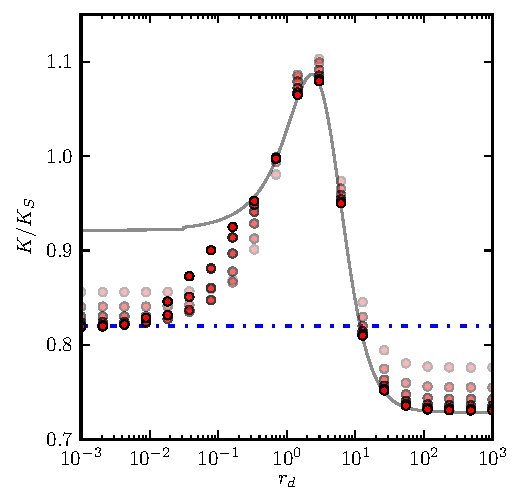
\includegraphics[width = 1 \textwidth]{plots/rb_cs.pdf}
    \end{figure}
\end{minipage}\begin{minipage}[t]{.5 \textwidth}
    \begin{figure}[H]
 %       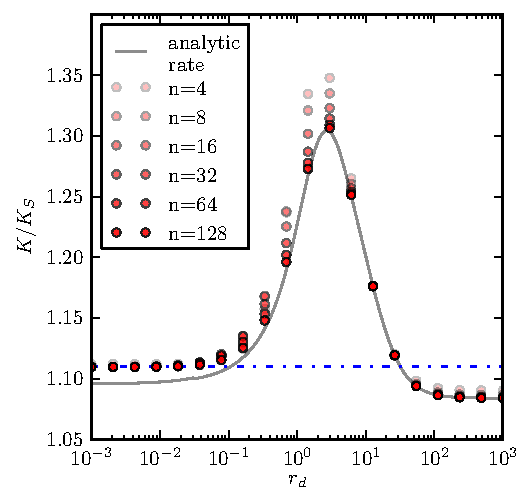
\includegraphics[width = 1 \textwidth]{plots/ab_cs.pdf}
    \end{figure}
\end{minipage}

\begin{minipage}[t]{1 \textwidth}
    \begin{figure}[H]
        \caption{Comparison of effective diffusivity profiles $D_{eff}(r)$ for attractive (blue) and repulsive (red) fluctuating barrier for different decay lengths $r_d$ resulting from different numeric approaches. A) gives results for density profiles calculated by numerical inversion of equation \eqref{Deff}. Necessary density profiles were obtained by the numerical Method of Lines for a smooth potential as given in \eqref{generalized_gaussian} with $U_2$, $a$, and $b$ as given in \eqref{Parameters}. B) gives results obtained from Brownian Dynamics simulations. Spatially resolved mean square displacement was calculated by radial binning of particles positions $\vec{x}$ for each time step, then integrating over $\Delta t$ and separately averaging over the particle square displacement $\Delta \vec{x}^{2}$ for each bin. The effective diffusivity was then calculated by \label{Deff_numeric}}
    \end{figure}
\end{minipage} \vspace{0.5 cm} \\

\subsection{Second Assumption}
%This section should bridge the gap from theory to experiments where measurements usually do not give any information of the detailed kinetics of the system but only show fluctuations as a potential of mean force and a spatially depending diffusivity profile.

\section{Summary}

\section{Summary}

\section{Conclusion}


\chapter{Appendix}
This part contains supplementary information that is too lengthy to be shown in the thesis itself.
\newpage
\section{Appendix A}
Analytic expression for Reaction Rate: \\
The decay length $r_d$ is substituted with $1/\alpha$ and the height of the barrier in units of the thermal energy of the particles $U_2/K_B T$ is substituted by $u$ to maintain a readable form of the results:
\begin{align}
    \frac{K}{K_{S}} &= \frac{F_1}{F_2}
    \label{two_state_rate}
\end{align}
with the nominator $F_1$ and denominator $F_2$ given by the following expressions:
\begin{align*}
    F_1 =& 2 \left(a \left(\alpha-5 b \alpha^2\right)+b \alpha-1\right) e^{2 \alpha (a+b)+u}-2 (a \alpha+1) (b \alpha-1) e^{2 (b+1) \alpha+u}-4 b \alpha (b \alpha+1) e^{3 a \alpha+b \alpha+u} \\
    &+2 b \alpha (b \alpha+1) e^{3 a \alpha+b \alpha+2 u}+4 b \alpha (b \alpha+1) e^{\alpha (a+b+2)+u}-2 b \alpha (b \alpha+1) e^{\alpha (a+b+2)+2 u} \\
    &-2 (a \alpha-1) (b \alpha+1) e^{4 a \alpha+u}+(a \alpha-1) (b \alpha+1) e^{4 a \alpha+2 u}-2 (a \alpha+1) (b \alpha+1) e^{2 (a+1) \alpha+u} \\
    &-(a \alpha+1) (b \alpha+1) e^{2 (b \alpha+u+\alpha)}-(3 a \alpha-1) (b \alpha+1) e^{2 (\alpha (a+b)+u)} \\
    &+(3 a \alpha+1) (b \alpha+1) e^{2 (a \alpha+u+\alpha)}-2 b \alpha (b \alpha+1) e^{\alpha (a+b+2)}+2 b \alpha (b \alpha+1) e^{\alpha (3 a+b)} \\
    &+e^{4 a \alpha} (a \alpha-1) (b \alpha+1)-e^{2 (a+1) \alpha} (a \alpha-1) (b \alpha+1)+(a \alpha+1) e^{2 (b+1) \alpha} (3 b \alpha-1) \\
    &-(a \alpha+1) (3 b \alpha-1) e^{2 \alpha (a+b)}, \\
    F_2 =& -4 \alpha \left(a^2 \alpha-a \alpha+a-b \alpha-2\right) e^{\alpha (a+b+2)+u}+2 \alpha \left(a^2 \alpha-a \alpha+a-b \alpha-2\right) e^{\alpha (a+b+2)+2 u} \\
    &-4 \alpha \left(a^2 \alpha-a (\alpha+1)+b \alpha+2\right) e^{3 a \alpha+b \alpha+u}+2 \alpha \left(a^2 \alpha-a (\alpha+1)+b \alpha+2\right) e^{3 a \alpha+b \alpha+2 u} \\
    &+2 \alpha e^{\alpha (a+b+2)} \left(a^2 \alpha-a \alpha+a-b \alpha-2\right)+2 \alpha e^{\alpha (3 a+b)} \left(a^2 \alpha-a (\alpha+1)+b \alpha+2\right) \\
    &-\left(3 \alpha^2 (a (b-2)+2 b)+\alpha (a-3 b+4)-1\right) e^{2 (\alpha (a+b)+u)} \\
    &-2 \left(\alpha^2 (a (5 b+2)-2 b)+\alpha (a+b-4)+1\right) e^{2 \alpha (a+b)+u} \\
    &+2 (a \alpha+1) ((b-2) \alpha+1) e^{2 (b+1) \alpha+u}+2 ((a-2) \alpha-1) (b \alpha+1) e^{2 (a+1) \alpha+u} \\
    &-2 (a \alpha-1) (b \alpha+1) e^{4 a \alpha+u}+(a \alpha-1) (b \alpha+1) e^{4 a \alpha+2 u}+((a+2) \alpha+1) (b \alpha+1) e^{2 (a \alpha+u+\alpha)} \\
    &-(a \alpha+1) ((3 b-2) \alpha+1) e^{2 (b \alpha+u+\alpha)}-e^{2 \alpha (a+b)} \left(\alpha^2 (a (3 b+2)-2 b)+\alpha (-3 a+b+4)-1\right) \\
    &+e^{4 a \alpha} (a \alpha-1) (b \alpha+1)-e^{2 (a+1) \alpha} ((3 a-2) \alpha-1) (b \alpha+1)+(a \alpha+1) e^{2 (b+1) \alpha} ((b+2) \alpha-1).
\end{align*}
\newpage
\section{Appendix B}
Analytic expressions for ininitely attractive and ininitely repulsive fluctuating barrier. \\
The decay length $r_d$ is substituted with $1/\alpha$ and the height of the barrier in units of the thermal energy of the particles $U_2/K_B T$ is substituted by $u$ to maintain a readable form of the results.
The limit of an infinitely attractive barrier of the expression for the reaction rate \eqref{two_state_rate} is the following:
\begin{equation}
    \lim_{u \rightarrow - \infty} = \frac{F_{1}^{-}}{F_{2}^{-}}
    \label{attractive_limit}
\end{equation}
with the nominator $F_1^-$ and denominator $F_2^-$ given by the following expressions:
\begin{align}
    F_1^- = &-2 b \alpha (b \alpha+1) e^{\alpha (a+b+2)}+2 b \alpha (b \alpha+1) e^{\alpha (3 a+b)} \nonumber \\
            &+e^{4 a \alpha} (a \alpha-1) (b \alpha+1) \nonumber \\
            &-e^{2 (a+1) \alpha} (a \alpha-1) (b \alpha+1)+(a \alpha+1) e^{2 (b+1) \alpha} (3 b \alpha-1) \nonumber \\
            &-(a \alpha+1) (3 b \alpha-1) e^{2 \alpha (a+b)} \\
    F_2^- = & 2 \alpha e^{\alpha (a+b+2)} \left(a^2 \alpha-a \alpha+a-b \alpha-2\right) \nonumber \\
            &+2 \alpha e^{\alpha (3 a+b)} \left(a^2 \alpha-a (\alpha+1)+b \alpha+2\right) \nonumber \\
            &-e^{2 \alpha (a+b)} \left(\alpha^2 (a (3 b+2)-2 b)+\alpha (-3 a+b+4)-1\right) \nonumber \\
            &+e^{4 a \alpha} (a \alpha-1) (b \alpha+1) \nonumber \\
            &-e^{2 (a+1) \alpha} ((3 a-2) \alpha-1) (b \alpha+1)+(a \alpha+1) e^{2 (b+1) \alpha} ((b+2) \alpha-1)
\end{align}

The limit of an infinitely repulsive barrier of the expression for the reaction rate \eqref{two_state_rate} is the following:
Ideal repulsive barrier:
\begin{equation}
    \lim_{u \rightarrow \infty} = \frac{F_1^+}{F_2^+}
    \label{repulsive_limit}
\end{equation}

with the nominator $F_1^+$ and denominator $F_2^+$ given by the following expressions:
\begin{align}
    F_1^+ = & (b \alpha+1) \left(-2 b \alpha e^{\alpha (a+b+2)}+2 b \alpha e^{\alpha (3 a+b)} \right. \nonumber \\
            &-(a \alpha+1) e^{2 (b+1) \alpha}+(1-3 a \alpha) e^{2 \alpha (a+b)} \nonumber \\
            & \left. +e^{4 a \alpha} (a \alpha-1)+e^{2 (a+1) \alpha} (3 a \alpha+1)\right) \\
    F_2^+ = & 2 \alpha e^{\alpha (a+b+2)} \left(a^2 \alpha-a \alpha+a-b \alpha-2\right) \nonumber \\
            &+2 \alpha e^{\alpha (3 a+b)} \left(a^2 \alpha-a (\alpha+1)+b \alpha+2\right) \nonumber \\
            &-e^{2 \alpha (a+b)} \left(3 \alpha^2 (a (b-2)+2 b)+\alpha (a-3 b+4)-1 \right) \nonumber \\
            &+e^{4 a \alpha} (a \alpha-1) (b \alpha+1) \nonumber \\
            &+e^{2 (a+1) \alpha} ((a+2) \alpha+1) (b \alpha+1)-(a \alpha+1) e^{2 (b+1) \alpha} ((3 b-2) \alpha+1)
\end{align}



\addcontentsline{toc}{section}{\numberline{}References}

\bibliography{Library.bib}{}
    \bibliographystyle{ieeetr}

\end{document}
